\documentclass[12pt]{report}
\usepackage{hepnicenames}
\usepackage{subcaption}
\usepackage{graphicx}
\usepackage[T1]{fontenc}
\usepackage[utf8]{inputenc}
\usepackage{titlepic}
\usepackage{hyperref}
\usepackage{gensymb}
\usepackage{subfiles}
\usepackage{siunitx}
\usepackage{makecell}
\usepackage[a4paper, margin=2cm]{geometry}
\usepackage{fourier}
\usepackage{tabularx}
\usepackage{array}
\usepackage{caption}
\usepackage{amsmath}
\usepackage{commath}
\usepackage{amssymb}
\usepackage{makecell}
\usepackage{braket}
\usepackage{physics}
\renewcommand\theadalign{bc}
\renewcommand\theadfont{\bfseries}
\renewcommand\theadgape{\Gape[4pt]}
\renewcommand\cellgape{\Gape[4pt]}

\title{Cosmic muon magnetic moment and lifetime.\\
	\large v1.4}

\author{Matei A.V. Climescu}
\date{Mainz, 2021}

\newenvironment{changemargin}[2]{%
\begin{list}{}{%
\setlength{\topsep}{0pt}%
\setlength{\leftmargin}{#1}%
\setlength{\rightmargin}{#2}%
\setlength{\listparindent}{\parindent}%
\setlength{\itemindent}{\parindent}%
\setlength{\parsep}{\parskip}%
}%
\item[]}{\end{list}}


\DeclareSIUnit\gauss{G}


\begin{document}
\maketitle
\begin{titlepage}
\begin{changemargin}{-0cm}{-0cm}
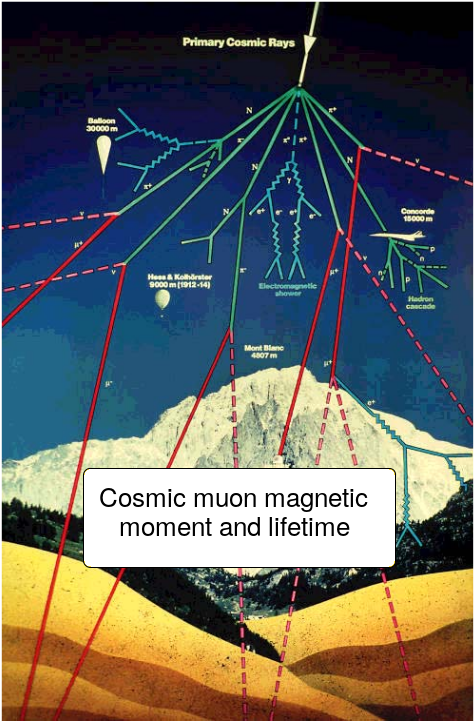
\includegraphics[width=\linewidth]{./fig/cover.png}
\end{changemargin}
\end{titlepage}


    
\chapter{Introduction}

This experiment is based on the Diplomarbeit of Mathias Heel in 1982 (\textit{Aufbau eines Versuchs im Fortgeschrittenen-Praktikum zur Messung der Lebendauer von Myonen}) and in particular the Staatsexamensarbeit of Joachim Geisb\"{u}sch in 1991 (Verbesserungen zum Experiment) at the University of Mainz's Departement of Physics. This experiment script was re-written in English by Matei Climescu in 2020 from Andreas Winhart's German version from 2001. The full script is available at \href{https://github.com/matclim/muonlifetime} and is publicly available for improvements, updates and changes there.



This experiment allows for the determination of the lifetime and magnetic moment of cosmic muons. Students can have a first introduction to elementary particle physics measurements and analysis methods with relatively simple means. 


The muon \Pmuon is an elementary particle often referred to as the electron's `heavy cousin'. It has identical properties to the electron and thus behaves in the same way, if the electron's mass was 207 times larger. The same can be said for the charged tau lepton \Ptauon (sometimes called the tauon) albeit with a 3491 mass factor instead. This gives rise to the concept of Lepton universality. The reason why the number of lepton generations is three remains unclear. Muons are of particular interest because:


\begin{itemize}
\item Parity violation in the weak sector is a particularly important part of modern physics: nature isn't invariant to spatial transformations, this is one of the results of the experiment.

\item A fairly accurate measurement for the weak coupling constant can be performed along with the muon's lifetime. The measurement of the anomalous magnetic moment of the muon, the so-called `g-2 factor' is an important test for the validity of QED.

\item Muons are the main component of sea-level cosmic radiation. The radiation density remains low however: the verticle flux of muons above \SI{1}{GeV/c}
\end{itemize}


    % !TEX root = Experiment41.tex

 
 \chapter{The Standard Model of Particle Physics}
 
 
 
After closer investigation of cosmic radiation, many new particles were discovered, such as neutral Kaons \PKzero in 1947, prompting Nobel prize Willis Lamb to declare ``The finder of a new elementary particle used to be rewarded by a Nobel Prize, but such a discovery now ought to be punished by a 10,000 dollar fine.''. As new techniques, such as particle accelerators, were improved, this `Particle Zoo' became more and more confusing to physicists. In the 1960s and 70s, a new model emerged: the Standard Model which brought order to the apparent chaos. It did so by articulating the phenomenology of known fundamental interactions into a single self-consistent, locally gauge-invariant quantum field theory centered around electromagnetism (Quantum Electro-Dynamics or \textit{QED}), the strong nuclear force (Quantum Chromo-Dynamics or \textit{QCD}) and the weak nuclear force.

Those interactions are mediated by spin-1 particles, the so called \textit{vector-bosons}: the photon \Pgamma mediates QED, eight massless but coloured gluons \Pgluon mediate QCD and three massive bosons \PZ, \PWpm mediate the weak interaction. Finally a single spinless massive \textit{scalar boson}, the so called \textit{Higgs Boson} was observed in 2012 and allows for massive bosons and at least certain fermions to be massive. All those bosons can be found in Table \ref{tab:bosons}. Each interaction takes place via the exchange of its bosons, for example, the $\beta^{-}$-decay of $^{137}\text{Cs}$ to $^{137}\text{Ba}$ can in fact be seen as a neutron's \Pdown emitting a \PWminus and thus becoming a \Pup, causing the neutron to become a proton. This reaction can be seen in Figure \ref{fig:betadecay}.
Matter however is made of fermions, particle with spin $\frac{1}{2}$, those, in the Standard Model are classified as \textit{quarks} and \textit{leptons}.
The Standard Model was observed to hold  6 massive quarks, reacting to all three interactions, 3 charged leptons, sensitive to electromagnetism and the weak interaction, and 3 neutral leptons, \textit{neutrinos}, which only interact through the weak interaction. They can be found in Table \ref{tab:SM}.

\begin{table}[htbp]
\centering
\resizebox{\linewidth}{!}{%
\begin{tabular}{|c|c|c|c|c|c|c|}
\hline
\textbf{Generation} & \multicolumn{2}{c|}{\textbf{1}} & \multicolumn{2}{c|}{\textbf{2}} & \multicolumn{2}{c|}{\textbf{3}} \\ \hline
& Fermion & Mass [MeV] & Fermion & Mass [MeV] & Fermion & Mass [MeV] \\ \hline
Up-type quarks ($q=\frac{2}{3}$) & up (\Pup) & $\sim 2.2$ & charm (\Pcharm) & $\sim 1300$ & top (\Ptop) & $173000 $  \\ \hline
Down-type quarks ($q=\frac{+2}{3}$) & down (\Pdown) & $\sim 4.7$ & strange (\Pstrange) & $\sim 95$ & beauty/bottom (\Pbottom) & $\sim 4200$ \\ \hline
Charged leptons ($q=\frac{-1}{2}$) & electron (\Pelectron) & $0.511$  & muon (\Pmuon) & $113$ & tau (\Ptauon) & $1780$  \\ \hline
Neutrinos ($q=0$) &  electron neutrino (\Pnue) & $\sim 0$ & muon neutrino (\Pnum) & $\sim 0$ & tau neutrino (\Pnut) & 0 \\ \hline
\end{tabular}}
\caption{Standard Model fermions.}
\label{tab:SM}
\end{table}

\begin{table}[htbp]
\centering
\scriptsize
\setlength\tabcolsep{2pt}
\begin{tabular}{|c|c|c|c|c|c|c|c|}
\hline
\textbf{Interaction} & \textbf{Boson} & \textbf{Mass [GeV]} & \textbf{Range [m]} & \textbf{Time scale [s]} & \textbf{spin} & \textbf{coupling} & \textbf{Fields} \\ \hline
Strong & gluon (\Pgluon)& 0 & $10^{-15}$ & $10^{-23}$ & 1 & $\sim 1$ & Quarks \\ \hline
Electromagnetic & photon (\Pgamma) & 0 & $\inf$ & $10^{-20}$ & 1 & $1/137$ & Electric charge \\ \hline
Weak & Z-zero boson (\PZzero), W bosons (\PWpm) & 91.2, 80.4 &  $\sim 10^{-17}$ & $10^{-8}$ & 1 & $10^{-5}$ & Quarks and leptons \\ \hline
Higgs & boson \PHiggs & $ 125.2$ & $\sim 10^{-18}$ &  $\sim 10^{-22}$ & 0 & variable & Massive fields \\ \hline
Gravity & graviton ($g$) & 0 & $\inf$ & - & 2 & $> 10^{-41}$ & Massive fields \\ \hline

\end{tabular}
\caption{Standard Model force carriers.}
\label{tab:bosons}
\end{table}


\begin{figure}[htbp]
\centering
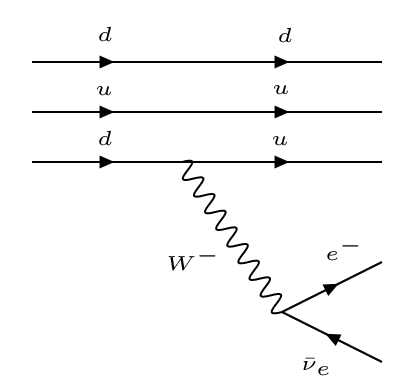
\includegraphics[width=0.5\linewidth]{./fig/betadecay.png}
\caption{Weak decay of a neutron to a proton.}
\label{fig:betadecay}
\end{figure}

Ordinary matter is overwhelmingly composed of first generation particles: \textit{up} and \textit{down}- type quarks and \textit{electrons}, a proton is notably composed of two up-type quarks and one down-type quark while a neutron is composed of a single up-type quark and two down-type quarks. It should be noticed that this is mostly due to the unstable nature of particles from Generation 2 and 3 (with the notable exception of neutrinos). Those particles will decay into lighter ones, it should be noted that, as a general rule, heavier particles decay faster and thus have a shorter lifetime. 


    
\chapter{Cosmic Radiation}

\section{History of cosmic radiation}

In 1785, Charles-Augustin de Coulomb discovered that charge was released by a charged electroscope over time. Over a century later, Wilson and Geitel discovered ionization currents using a bell apparatus shown in Figure \ref{fig:bell}. They noticed that a dark current persisted in the bell and that, despite it being weakened by covering the apparatus in lead, it could never quite be eliminated, leading them to postulate the existence of telluric radioactivity (or Earth radioactivity).

\begin{figure}[htbp]
\centering
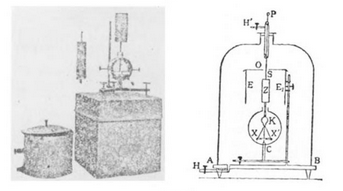
\includegraphics[width=0.6\linewidth]{./fig/bell.png}
\caption{Geitel's ionization current apparatus (1900).}
\label{fig:bell}
\end{figure}

It wasn't until 1912 that it was determined that the source of this ``dark current'' couldn't be the earth: Victor Hess experimented with putting an electroscope onto a balloon which he launched to an altitude of up to \SI{5300}{\meter}. He found that the rate of radiation was there some three times what it was at sea level and this, allied with his experimentation during a partial solar eclipse, allowed him to rule out the Sun as the source of this myterious radiation, enabling him to discover a natural source of high-energy particles: cosmic rays, awarding him the Nobel prize in 1936. Later studies from Freier, Lofgren, Ney, Oppenheimer, Bradt and Peters from 1948 and many others accross the years showed the existence of different radiation in the upper atmosphere, the so-called primary radiation, composed of around $90\%$ protons and around $10\%$ other nuclei which corresponds to the material ratio found in your average star, leading to the conclusion that cosmic radiation was mostly emitted by stars.

\section{Primary cosmic rays}

In star explosions, such as Supernovae, electric fields arise at the star's surface, this implies the acceleration of charged particles to very high energies. Particles thus gain enough energy to exit the star's potential well but whether they actually are able to be emitted is also dependent on their mass: lighter particles such as \Pelectron see their energy quickly depleted through \textit{bremsstrahlung emissions}. This is due to the way the emitted bremsstrahlung energy $E_\text{Brems}$ evolves relative to the emitting particle's mass $m_\text{P}$:

\begin{equation}
E_\text{Brems}	\propto \frac{1}{m_\text{P}^2}.
\end{equation}

This implies that protons and heavy nuclei are the main constituents of what exits the star.

When this primary radiation enters the atmosphere, it's deflected by the Earth's B-field via the Lorentz force. At our latitude (50\degree -Mainz Gutenbergplatz), particles require at least \SI{3}{\giga\electronvolt} to enter the atmosphere. This values varies around the globe and is in particular lower near the poles since there is a higher proportion of field lines parralel to the Earth's surface. This is often called the \textit{magnetic latitude effect} shown in Figure \ref{fig:magintensity}.


\begin{figure}[htbp]
\centering
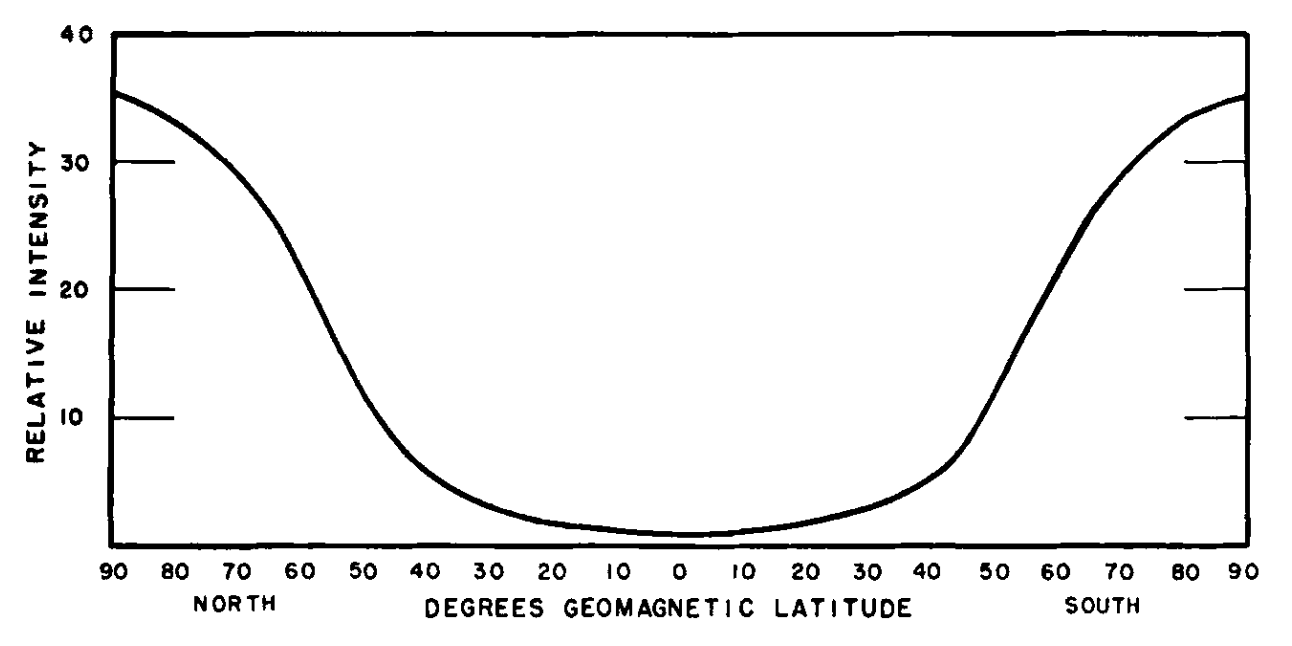
\includegraphics[width=0.8\linewidth]{./fig/intensity.png}
\caption{Magnetic latitude effect at sea level.}
\label{fig:magintensity}
\end{figure}

The Earth's $\mathbf{B}$-field is a dipole field with magnetic moment of $8.1 \cdot 10^{18}\text{ J}.\text{G}^{-1}$. The critical momentum, the minimal momentum needed to breach the atmosphere is given by:

\begin{equation}
\text{P}_\Phi=1.5\cdot 10^{10} \cos^4\Phi |z| \text{ eV}.c^{-1}.
\end{equation}

where $z$ is the particle's charge in units of elementary charge. The discrenpency in the number of positive and negative particles results in an east-west asymmetry in particle intensity. At least $90\%$ of the primary particles have a positive charge as shown in Figure \ref{fig:assym}.

\begin{figure}[htbp] %No better figure could be found, it could be remade%
\centering
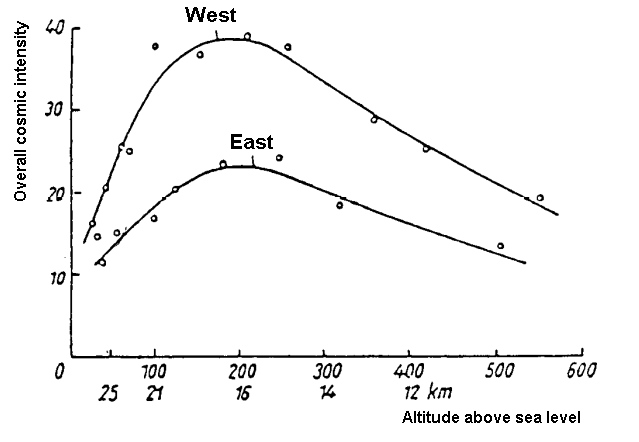
\includegraphics[width=0.8\linewidth]{./fig/assym.png}
\caption{East-west asymmetry measured at different altitudes.}
\label{fig:assym}
\end{figure}


\section{Secondary comic rays}

Since the atmosphere is a matter-rich environment, it provides any entering primary radiation with fields to interact with, which gives rise to a variety of processes, producing so-called \textit{secondary cosmic rays}. Low energy protons, with momenta up to \SI{10}{\giga\electronvolt} knock-off individual nucleons from nitrogen and oxygen nuclei. At higher energy, nuclear (meson-dominated) bremsstrahlung radiation is the main source of energy loss. An example of it can be found in Figure \ref{fig:scat}. 

\begin{figure}[htbp]
\centering
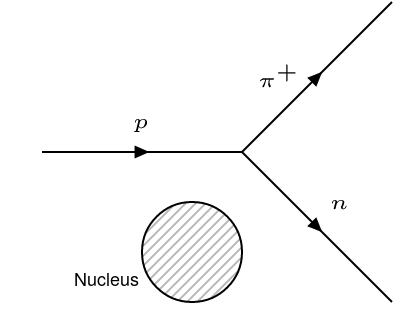
\includegraphics[width=0.5\linewidth]{./fig/nscat.png}
\caption{Bremsstrahlung pion emission from proton-nucleus scattering.}
\label{fig:scat}
\end{figure}






The produced mesons are mostly pions but heavier flavour particles can be created at energies above \SI{100}{\giga\electronvolt} such as Kaons.

Protons from primary cosmic rays have an energy up to a couple PeV and will thus also perform nucleon-antinucleon pairs. This energy level remains very rare however as can be seen in Figure \ref{fig:knee}

\begin{figure}[htbp]
\centering
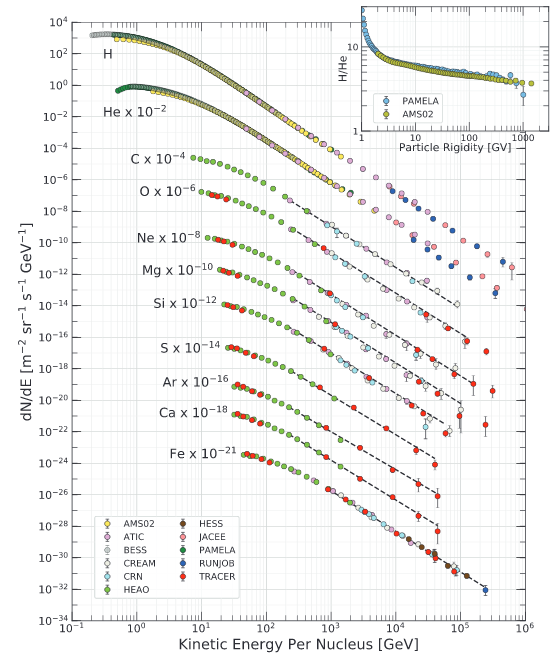
\includegraphics[width=\linewidth]{./fig/knee.png}
\caption{Fluxes of nuclei of the primary cosmic radiation in particles per-energy-per-nucleus are plotted vs energy-per-nucleus. The inset shows the H/He ratio at constant rigidity \cite{Tanabashi:2018oca}.}
\label{fig:knee}
\end{figure}

The number N of protons for a given energy is given by:

\begin{equation*}
\text{N}(E)=K\cdot E^{-\gamma}.
\end{equation*}

where $K$ is a constant and $\gamma$ varies with the energy: from $\gamma=1$ for $E=\SI{10}{\giga\electronvolt}$ to $\gamma=2.5$ for very high energies \cite{Tanabashi:2018oca}.

For our purpose, pions are of particular interest. Charged pions decay overwhelmingly ($\sim 99.99\%$) into a muon and a muon neutrino with a lifetime of $2.6 \cdot 10^{-8} \text{ } \si{\second}$ \cite{Tanabashi:2018oca}:

\begin{equation*}
\Ppiplus \rightarrow \APmuon + \Pnum \text{ and } \Ppiminus \rightarrow \Pmuon + \APnum.
\end{equation*}

Because of their relatively low energy loss and long lifetimes, nearly all muons reach the Earth's surface.

\section{Cosmic radiation content}

There are three main components to cosmic radiation: so-called \textit{hard-radiation}, \textit{soft-radiation} and \textit{nuclear-radiation}. A sketch of cosmic radiation and it's content can be found in Figure \ref{fig:cos}.

\begin{figure}[htbp]
\centering
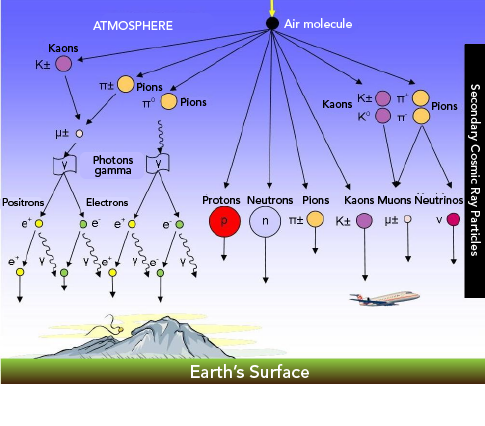
\includegraphics[width=0.7\linewidth]{./fig/Cosmic_ray_scattering.png}
\caption{Cosmic rays and their components. On the left is the soft component, in the middle is the nuclear component and on the right is the hard component \cite{LTSCA}.}
\label{fig:cos}
\end{figure}

\subsection{Nuclear radiation}

As its name implies, nucleons and light atomic nuclei make up nuclear cosmic radiation. Atomic nuclei lose energy through absorption into the air while low energy protons lose theirs through ionization. Neutrons interact abundently with atmospheric nuclei through elastic scattering which creates a gain in thermal energy in said nuclei. The proportion of nuclear radiation reaching the earth's surface is negligible.

\subsection{Soft radiation}

\Pgamma and \Pepm are the constituents of soft cosmic radiation. Electrons arise partially from muon decays but mostly from photon pair creation. Those are mostly produced in two ways: electromagnetic bremsstrahlung/Cherenkov radiation and from the decay of neutral pions \Ppizero. Neutral pions are produced as part of nuclear cosmic radiation and decay into photon pairs with a $8.52 \cdot 10^{-17}\text{ }\si{\second}$ lifetime \cite{Tanabashi:2018oca}. Said photons will overwhelmingly decay into \Pepm pairs if they have an energy $E>2m_{\Pe}$.

\begin{equation*}
\Ppizero\rightarrow\Pgamma\Pgamma,\text{   }\gamma\rightarrow\APelectron\Pelectron,\text{   }\Pepm\rightarrow\Pepm\Pgamma,\text{   }\Pgamma\rightarrow\APelectron\Pelectron \text{   etc.}.
\end{equation*}


The pion's energy will thus be distributed over many particles until a so-called \textit{critical energy} is reached. Under said energy, ionization, as opposed to particle creation, becomes the dominant energy loss mechanism which signals the end of the shower as the number of particles will thus quickly decrease. \Pgamma lose energy through the Compton and photoelectric effects which implies that those remaining particles can easily be shielded by a couple centimetres of lead.

\subsection{Hard radiation}

The hard radiation component is revolves around heavy flavour leptons, mainly \Pmu flavour ones. Due to their relatively high mass, muons only lose small amounts of energy due to bremsstrahlung and mostly through ionization since they have a very high critical energy ($\sim \SI{3.6}{\TeV}$). The energy loss of massive charged particles is described by the \textit{Bethe-Bloch Formula}:

\begin{equation}
-\od{E}{x}=\frac{4\pi n z^2 e^4}{m_{\Pe}}\Big(\text{ln}(\frac{2m_{\Pe}v^2}{I(1-\beta^2)}-\beta^2)  \Big).
\end{equation}

where $E$ is the energy, $x$ the distance, n is the number of electrons per $\text{cm}^3$ in the traversed material, $z \cdot e$ is the electrical charge and $v$ the particle's speed, $I$ is the mean excitation potential of an atom in the material, often approximated by $I\simeq 17.7 Z^{0.85}$ and $\beta$ is the factor $\beta = \frac{v}{c}$. This distribution has its minimum for particles which have a $\beta\gamma \sim 3$ with $\gamma=\frac{1}{\sqrt{1-\beta^2}}$ irrespective of the particle as shown in Figure \ref{fig:BB}. Particle which have such an energy or slightly above it are called \textit{Minimum-Ionizing-Particles} (MIPs).

\begin{figure}[htbp]
\centering
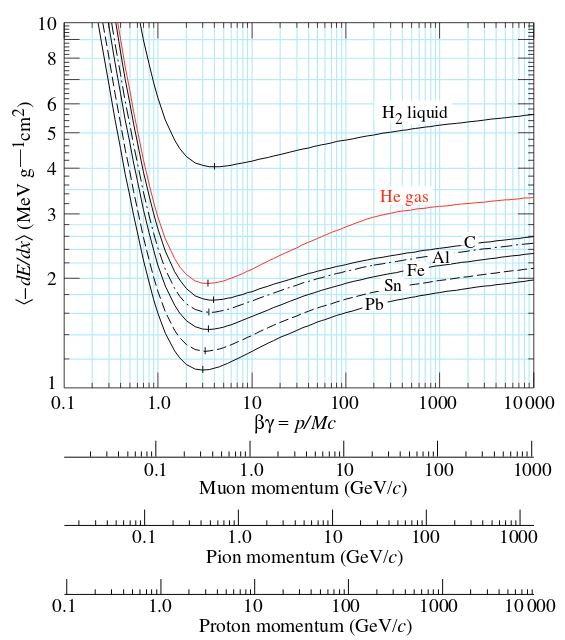
\includegraphics[width=0.7\linewidth]{./fig/BB.png}
\caption{Mean energy loss rate in liquid (bubble chamber) hydrogen, gaseous helium, carbon,aluminum, iron, tin, and lead. Radiative effects, relevant for muons and pions, are not included.These become significant for muons in iron for $\beta\gamma \gtrsim 1000$, and at lower momenta for muons in higher-Z absorbers \cite{Tanabashi:2018oca}.}
\label{fig:BB}
\end{figure}


The energy loss for a MIP in air is $\sim 1.8 \text{ MeV per g/cm}^2$, the number of particles $N$ with energy $E_0$ is given by the integration:

\begin{equation}
N=\int_0^{E_0}\od{E}{E/\text{d}x}.
\end{equation}


When considering the finite number of muons at a given energy and their lifetime of $\tau\sim\SI{2.2}{\micro\second}$, it could be expected that a muon travels a minimum of $\sim \SI{600}{\meter}$ on average in vacuum. If time dilation is accounted for however, the muon's lifetime and thus it's travel distance are increased by a factor $\Pgamma$:

\begin{equation}
\tau_{\Pmu\text{Lab}}=\gamma\tau_{\Pmu}.
\end{equation}

As an example, muons with an energy of \SI{3}{\giga\electronvolt} will have a $\gamma=\frac{E}{m}=\frac{\SI{3}{\giga\electronvolt}}{\SI{105}{\mega\electronvolt}}\sim 29$ leading to a lifetime $\tau \sim \SI{62}{\micro\second}$. It would thus travel $\sim \SI{20}{\kilo\meter}$ in vacuum which corresponds to the approximate height of formation of muons in the atmosphere from pion decays. High-energy muons can make it to the earth's surface almost unhindered and easily pierce through \SI{500}{\meter} of water.

This, in addition to magnetic deflection are the main reasons why the muon momentum-spectrum ($N(E)=\frac{K}{E^{\Pgamma}}$) at ground level is shifted towards high energies as shown in Figure \ref{fig:shift}.

\begin{figure}[htbp]
\centering
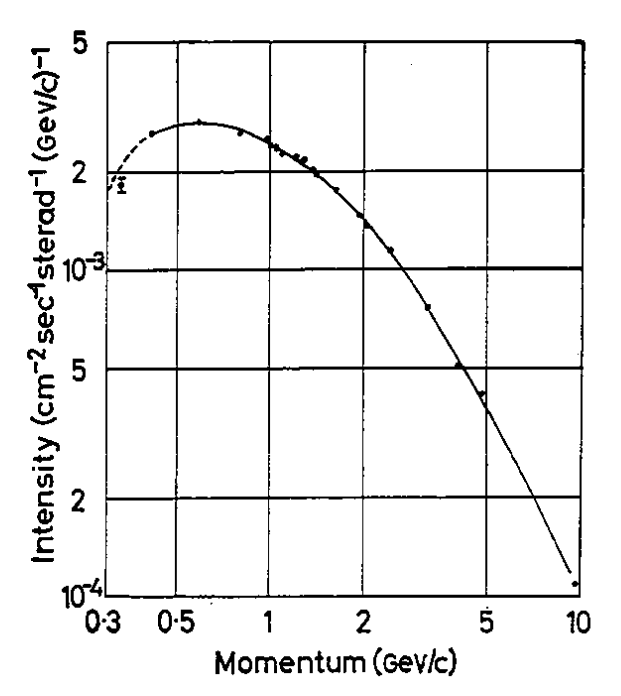
\includegraphics[width=0.5\linewidth]{./fig/shiftDur.png}
\caption{Vertical differential momentum of muons at $54^\circ$ \cite{Gardener_1962}.}
\label{fig:shift}
\end{figure}


\section{Cosmic ray intensity}

In order to perform the experiment, it is necessary to know the width of each cosmic component, especially muons. Table \ref{tab:flx} shows the muon flux as a function of relevant parameters. Figure \ref{fig:cosflux} indicates the flux of various particle productions for different altitudes. At our latitude the muon asymmetry is about 1.3.

\begin{table}
\centering
\tiny
\begin{tabular}{|c|c|c|c|c|c|c|c|c|c|c|c|c|c|}
\hline
\multicolumn{5}{ |c| }{Altitude} & \multicolumn{3}{ |c| }{Total intensity} &\multicolumn{3}{ |c| }{Hard component} &\multicolumn{3}{ |c| }{ Soft Component} \\ \hline
\multicolumn{2}{ |c| }{Distance} & \multicolumn{3}{ |c| }{Pressure} & \makecell{Omni-\\direct-\\ional} & \makecell{Verti-\\cal} & \makecell{Latitude\\effect} & \makecell{Omni-\\direct-\\ional} & \makecell{Verti-\\cal} & \makecell{Latitude\\effect} & \makecell{Omni-\\direct-\\ional} & \makecell{Verti-\\cal} & \makecell{Latitude\\effect} \\ \hline
metres & feet & \si{\milli\meter} Hg & atm & \si{\meter} H$_2$O & \makecell{particle \\ \si{\per sea\cdot\cm\square}} & \makecell{particle \\ \si{\per sea\cdot\cm\square}\\\si{\cdot sterad}} & $\%$ & \makecell{particle \\ \si{\per sea\cdot\cm\square}} & \makecell{particle \\ \si{\per sea\cdot\cm\square}\\\si{\cdot sterad}} & $\%$ &\makecell{particle \\ \si{\per sea\cdot\cm\square}} & \makecell{particle \\ \si{\per sea\cdot\cm\square}\\\si{\cdot sterad}} & $\%$ \\ \hline
0 & 0 & 760 & 1.000 & 10.33 & 0.020 & 0.015 & 10 & 0.013 & 0.000 & 10 & 0.007 & 0.000 & 10 \\
2000 & 6561 & 59.6 & 0.781 & 8.11 & 0.033 & 0.025 & 16 & 0.018 & 0.012 & 15 & 0.017 & 0.013 & 15 \\
4500 & 14764 & 43.3 & 0.870 & 5.59 & 0.10 & 0.07 & 25 & 0.08 & 0.020 & 25 & 0.07 & 0.06 & 25 \\
10000 & 32808 & 10.8 & 0.201 & 2.60 & 0.7 & 0.3 & 45 & 0.10 & 0.05 & 30 & 0.6 & 0.25 & 30 \\
16100 & 52822 & 7.60 & 0.100 & 1.04 & 1.5 & 0.5 & 75 & 0.23 & 0.08 & ? & 1.25 & 0.42 & 80 \\
30000 & 98425 & 0.87 & 0.0115 & 0.118 & 0.5 & 0.15 & 83 & 0.4 & 0.13 & ? & 0.06 & 0.02 & ? \\
$\infty$ & $\infty$ & 0 & 0 & 0 & 0.3 & 0.1 & 00 & ? & ? & ? & ? & ? & ? \\ \hline
\end{tabular}
\caption{Cosmic rays intensity at 50$^\circ$.}
\label{tab:flx}
\end{table}

\begin{figure}[htbp]
\centering
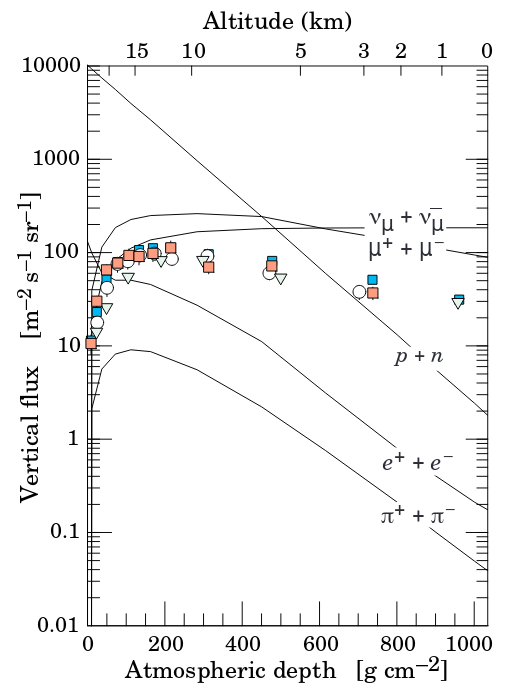
\includegraphics[width=0.5\linewidth]{./fig/cosflux.png}
\caption{Vertical fluxes of cosmic rays in the atmosphere with $E>\SI{1}{\giga\electronvolt}$ estimated from the nucleon flux. The points show measurements of negative muons with $E_{\Pmu} > \SI{1}{\giga\electronvolt}$ \cite{Tanabashi:2018oca}.}
\label{fig:cosflux}
\end{figure}



    

\chapter{The muon}

\section{Muon history}

Muons were discovered by Carl David Anderson and his student Seth Neddermeyer at Caltech in 1936 while they were working on cosmic rays. They observed that certain particles had a much more curved trajectory in their cloud chamber, than electron but less than protons. They were curving in the same direction as electrons meaning they had the same charge. They were initially mistaken for Yukawa's pion which supposedly mediated the strong interaction but were discovered not to have the right properties as it didn't interact strongly as it could traverse thick plates of metal unhindered. Heisenberg and Euler made the first computation of its lifetime in 1938, through the decreasing intensity as a function of travel distance. In 1947, Powell, Lattes, Muirhead and Ochialini used emulsion plates to discover two different ``mesons'': the \Ppi-meson and the \Pmu-meson (which was later revealed to be quite different from its counterpart).

\section{Muon production from pion decays}

Pions are the lightest hadron and thus can only decay electroweakly, they are, as $\Pquark\APquark$ with antiparallel spins, spinless bound-states. Since they can only decay to fermions, which have spin $\frac{1}{2}$, only even-number-body-decays are allowed by angular momentum conservation laws. In addition, because of flavour conservation laws, leptons need to be produced as pairs or together with a(n) (anti)neutrino. An example pion decay is given in Figure \ref{fig:piedec}.


\begin{figure}[htbp]
\centering
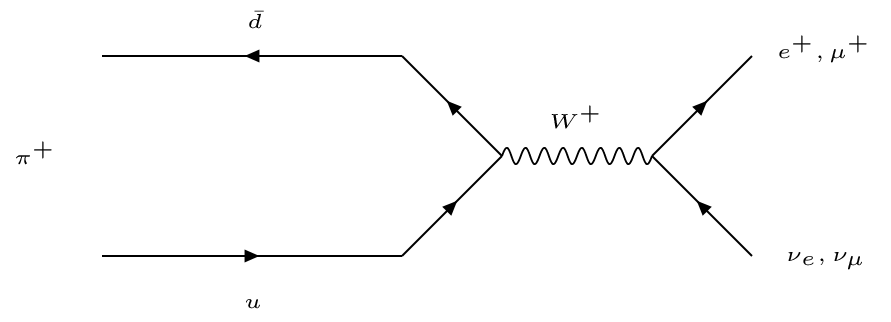
\includegraphics[width=0.7\linewidth]{./fig/pideac.png}
\caption{Positive pion decay.}
\label{fig:piedec}
\end{figure}

There are thus 4 channels available for pions to decay:

\begin{equation*}
\Ppiplus \rightarrow \APelectron \Pnue \text{;\hspace{3cm}}\Ppiminus \rightarrow \Pelectron \APnue;
\end{equation*}

\begin{equation*}
\Ppiplus \rightarrow \APmuon \Pnum \text{;\hspace{3cm}}\Ppiminus \rightarrow \Pmuon \APnum.
\end{equation*}

This gives rise to the branching ratio:

\begin{equation}
R=\frac{\text{Rate}(\Ppi\rightarrow \Pe \Pnu)}{\text{Rate}(\Ppi\rightarrow \Pmu \Pnu)} = (1.230 \pm 0.004) \cdot 10^{-4}.
\end{equation}

Muon-channel decays are thus nearly 10000 times more likely than electron-channel decays. This might be surprising when looking at energy phase space consirations: the muon being around 207 times heavier than the electron, the phase space would thus be:

\begin{equation}
R_{\text{phase-space}}=\frac{1-\big(\frac{m_{\Pe}}{m_{\Ppi}}\big)^2}{1-\big(\frac{m_{\Pmu}}{m_{\Ppi}}\big)^2} \simeq 2.35.
\end{equation}

with $m_{\Ppi} = 273 m_{\Pe}$.

This wrong prediction is due to the lack of account taken from \textit{V-A Coupling}, the combination of a vector (such as flight direction) and an axial vector (such as momentum) in the weak decay. This requires a new quantum number to be introduced: \textit{Helicity H}, which is defined as the projection of spin on momentum:

\begin{equation*}
H\doteq \vec{s}\cdot \hat{p} \text{\hspace {1cm} with \hspace{1cm}} \hat{p}=\frac{\vec{p}}{|\vec{p}|}.
\end{equation*}

Helicity  expectation and alignement value are defined by:

\begin{equation*}
\Braket{H}\doteq\pm\frac{v}{c}.
\end{equation*}

With the expectation taking negative values for particles (\Pelectron, \Pmuon,\Pnue,\Pnum) and positive ones for antiparticles (\APelectron,\APmuon,\APnue,\APnum). It should be noted that in the Standard Model, only \text{left-handed} ($\Braket{H}=-1$, spin and momentum antiparallel) neutrinos and thus only \textit{right-handed} ($\Braket{H}=+1$, spin and momentum parallel) antineutrinos exist. Neutrinos can be seen as practically massless and thus always travelling at the speed of light. This implies, through momentum and angular momentum conservation,that pions can only decay in certain configurations such as that shown in Figure \ref{fig:helipi}.

\begin{figure}[htbp]
\centering
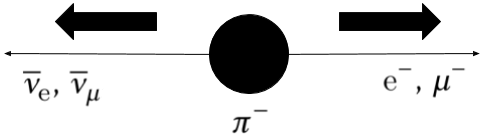
\includegraphics[width=0.7\linewidth]{./fig/helipi2.png}
\caption{Spin and momentum in a negative pion's decay, as seen in the pion's rest frame.}
\label{fig:helipi}
\end{figure}

Since the pion is spinless, the neutrino and charged fermion need to have opposite spin, since antineutrinos can only have right-handed helicity, the muon is emitted with right-handed helicity. However, only left-handed particles participate in the weak interaction. This can be seen in the right-handed helicity solution of the Dirac equation:

\begin{equation}
u_{\uparrow}=N\begin{pmatrix} \cos{\frac{\theta}{2}} \\ e^{i\phi}\sin{\frac{\theta}{2}} \\ \frac{|\vec{p}|}{E+m}\cos{\frac{\theta}{2}} \\ \frac{|\vec{p}|}{E+m}e^{i\phi}\sin{\frac{\theta}{2}} \end{pmatrix}.
\end{equation}

The left-handed chirality projector is given by:

\begin{equation}
P_{\text{L}}=\frac{1}{2}(1-\gamma^5)=\frac{1}{2} \begin{bmatrix} 1 & 0 & -1 & 0 \\
0 & 1 & 0 & -1 \\
-1 & 0 & 1 & 0 \\
0 & -1 & 0 & 1 \end{bmatrix}.
\end{equation} 

with, when applied to the spinor yields:

\begin{equation}
P_{\text{L}}u_{\uparrow}=\frac{N}{2}\Big(1-\frac{|\vec{p}|}{E+m}\Big)u_{\text{L}}.
\end{equation} 

which tends to zero in the limit $m<<E$, while

\begin{equation}
P_{\text{R}}u_{\uparrow}=\frac{N}{2}\Big(1+\frac{|\vec{p}|}{E+m}\Big)u_{\text{R}}.
\end{equation}

tends to $u_{\text{R}}$ in the limit $m<<E$. This leads to

\begin{equation}
u_{\uparrow}=P_{\text{R}}u_{\uparrow} + P_{\text{L}}u_{\uparrow} = \frac{1}{2}\Big(1+\frac{|\vec{p}|}{E+m}\Big)u_{\text{R}} + \frac{1}{2}\Big(1-\frac{|\vec{p}|}{E+m}\Big)u_{\text{L}}.
\end{equation}

in the limit $E>>m$, the right-handed chiral and helicity states are identical as expected. Even though only left-handed chiral particles participate in the weak interaction, the right-handed contribution isn't necessarily zero. The matrix element is expected to be proportional to the left-handed chiral component of the right-handed helicity fermion spinor:

\begin{equation}
\text{M}_{fi} \propto \frac{1}{2} \Big(1-\frac{|\vec{p}|}{E+m}\Big) = \frac{m}{m_{\Ppi}+m} .
\end{equation}

The calculation of the branching ratio

\begin{equation}
R=\frac{P(\Ppi\rightarrow \Pe \Pnu)}{P(\Ppi\rightarrow \Pmu\Pnu)}\simeq \frac{m_{\Pe}^2}{m_{\Pmu}^2}\frac{(1-\frac{m_{\Pe}^2}{m_{\Ppi}^2})^2}{(1-\frac{m_{\Pmu}^2}{m_{\Ppi}^2})^2} \simeq 1.283 \cdot 10^{-4}.
\end{equation}

Which is in good agreement with experimental observations. For this measurement, it is necessary that muon in the pion rest-frame be entirely left-handed. The Lorentz transform into the Lab-frame allows for this in this experiment.

\section{Muon polarization in cosmic rays}

In this experiment, muons will be stopped in a \SI{25}{mm} thick copper plate. If other present materials are accounted for, such as the lead shielding, concrete ceilling and \SI{20}{\km}, only ``slow'' muons, with an energy estimated to be of $\sim\SI{609}{\mega\electronvolt}$ are actually stopped in the copper. While this might be an estimate, Figure \ref{fig:mupol} demonstrates the relative constance of polarization at energies between \SI{300}{\mega\electronvolt} and \SI{900}{\mega\electronvolt}.

\begin{figure}[htbp]
\centering
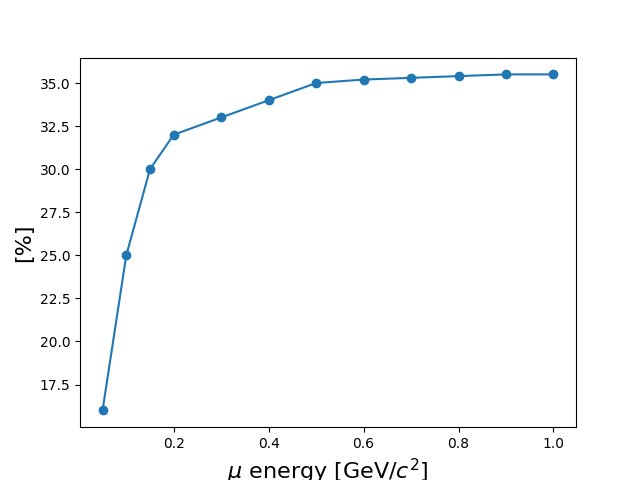
\includegraphics[width=0.7\linewidth]{./fig/muonpol.png}
\caption{Muon polarization as a function on energy.}
\label{fig:mupol}
\end{figure}

Muons of such energies can be created in two different ways (in the following, positive muons will be looked at):

\begin{itemize}

\item They can be produced in \SI{616}{\mega\electronvolt} pions and are then emitted in the direction of flight, with negative helicity and upward-facing spin (Figure \ref{sfig:spindeca}).

\item They can be produced in \SI{1058}{\mega\electronvolt} pions and are then emitted against the direction of flight, with positive helicity and downward-facing spin (Figure \ref{sfig:spindecb}).

\end{itemize}

\begin{figure}[htbp]
\centering
\caption{Muon polarization as a function on energy.}
\end{figure}

\begin{figure}[htbp]
  \centering
   \begin{subfigure}[t]{0.49\linewidth}
  \centering
   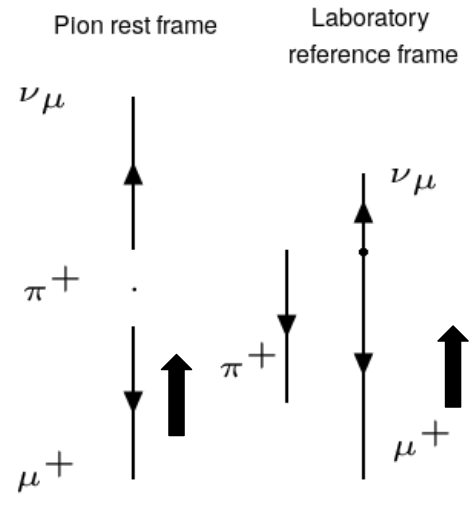
\includegraphics[width=0.7\linewidth]{./fig/spindecaa.png}
  \caption{}
\label{sfig:spindeca}
  \end{subfigure}
 \begin{subfigure}[t]{0.49\linewidth}
  \centering
   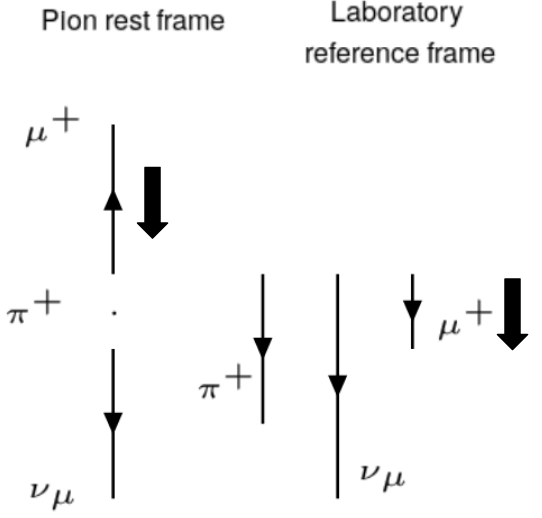
\includegraphics[width=0.7\linewidth]{./fig/spindecbb.png}
  \caption{}
  \label{sfig:spindecb}
  \end{subfigure}
  \caption{Production of \SI{609}{\mega\electronvolt} in cosmic radiation with (a) negative helicity and (b) positive helicity.}%
  \label{fig:spindec}
\end{figure}

With a uniform pion energy distribution, it was first impossible to observe polarized muons. At the aforementionned energy ranges however, the pion abundance as a function of energy $N(E)$ can be seen to display the following behaviour:

\begin{equation}
N(E) \mathrm{d}E \sim E^{-1.4}\mathrm{d} E.
\end{equation}

Thus the ratio of muons with positive helicity $N(\downarrow\uparrow)$ to those with negative helicity $N(\uparrow\uparrow)$ is:

\begin{equation}
\frac{N(\downarrow\uparrow)}{N(\uparrow\uparrow)}=\frac{616^{-1.4}}{1058^{-1.4}}\simeq \frac{2.15}{1}.
\end{equation}

An excess of muons with negative helicity is thus of polarization is expected. The polarization $P$ is defined as:

\begin{equation}
P\doteq \frac{N(\downarrow\uparrow)-N(\uparrow\uparrow)}{N(\downarrow\uparrow)+N(\uparrow\uparrow)}.
\end{equation}

It is thus expected to find a muon polarization of about $37\%$.

\section{Muon decays}

Muons decay with an average lifetime of $2.2 \cdot 10^{-6}\si{\second}$ into the lighter flavoured lepton, the electron. Since muons are stopped in copper and that the process is different for positive and negative muons, both processes will be treated separately.

\subsection{The decay of free \APmuon}

Positive muons remain in the free interstices and can thus decay like free muons. In order to preserve lepton number, the following decay takes place:

\begin{equation*}
\APmuon \rightarrow \APelectron + \Pnue + \APnum.
\end{equation*}

As a three-body decay, the positron's momentum spectrum is continious, however, due to the parity-violating nature of the weak interaction, an asymmetry in the positron's angular distribution can be found as shown in Figure \ref{fig:angassy}

\begin{figure}
\centering
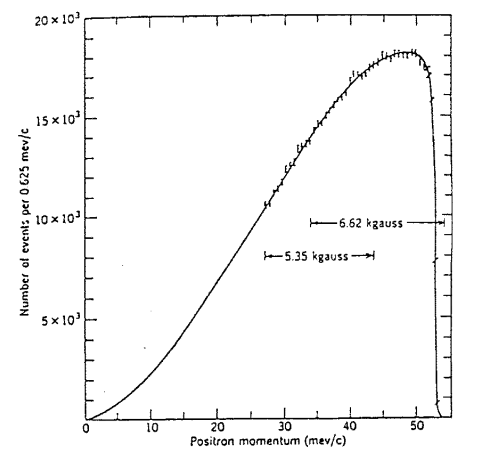
\includegraphics[width=0.5\linewidth]{./fig/posangas.png}
\caption{Final state positron from muon decays momentum spectrum.}
\label{fig:angassy}
\end{figure}

For the transition probability $W$ for the solid angle $\Omega$:

\begin{equation}
\label{eq:e413}
\mathrm{d}W=\frac{G_{\text{F}}^2m_{\Pmu}^5c^4}{192\pi^3\hbar^7}\big[2\epsilon^2(3-2\epsilon) \big] \Bigg[1+\frac{1-2\epsilon}{3-2\epsilon} \cos{\Theta} \Bigg] \Bigg[ \frac{1-n_{\Pe}s_{\Pe}}{2}\Bigg]\mathrm{d}\epsilon \frac{\mathrm{d}\Omega}{4\pi},
\end{equation}

with $\epsilon = \frac{E_{\Pe}}{E_{\text{max}}}$, $E_{\text{max}} = \frac{1}{2m_{\Pmu}c^2}$ and $\Theta$ the angle between the muon's spin and the positron's momentum. The first block between brackets provides the positron momentum spectrum, the second provides the angular distribution and the third represents the positron helicity in the V-A description. The third block can be approximated with $\frac{v_{\text{pos}}}{c} \sim 1$ and thus can be neglected. For the number of positron emitted at an angle $\Theta$ one can write:

\begin{equation}
N(\Theta)\sim 1+ a\cos{\Theta} \text{ with the assymmetry factor } a=\frac{1-2\epsilon}{3-2\epsilon}.
\end{equation}

The average assymmetry over all energies can be integrated from Equation \ref{eq:e413}:

\begin{equation}
N(\epsilon) \sim \int_0^1 \big[2\epsilon^2(3-2\epsilon) \big] \Bigg[1+\frac{1-2\epsilon}{3-2\epsilon} \cos{\Theta} \Bigg] \mathrm{d}\epsilon \implies N(\Theta)\sim 1 + \frac{1}{3}\cos{\Theta}.
\end{equation}

This corresponds to an assymmetry of $\sim 33\%$. This is illustrated in Figure \ref{fig:emassy}.

\begin{figure}[htbp]
\centering
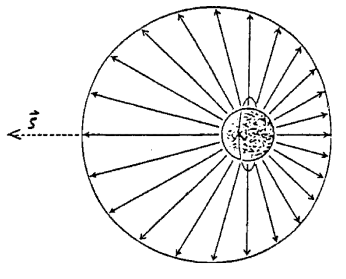
\includegraphics[width=0.7\linewidth]{./fig/emassy.png}
\caption{Illustration of positron angle emission in muon decays. The length of the arrow is proportional to the emission probability for that angle.}
\label{fig:emassy}
\end{figure}

In order for them to be detected, the positrons first need to exit the copper plate which, depending on their emission angle and the decay vertex position, requires a minimal energy of \SI{30}{\mega\electronvolt}. This leads to an assymmetry factor $a=0.38\pm0.04$ \cite{Heel}. The oberserved assymmetry in this measurement also depends on the Polarization $P$ of the muon:

\begin{equation}
\label{eq:larg}
N(\Theta)\sim1+aP\cos{\Theta}.
\end{equation}

The last remaining unknown if the muon's lifetime $\tau_{\Pmu}$. Integrating Equation \ref{eq:e413} over space and energy provides the transition probability $W$ which is nothing else than the \textit{inverse lifetime}:

\begin{equation}
W=\frac{G^2_{\text{F}}2m_{\Pmu}^5c^4}{192\pi^3\hbar^7}=\frac{1}{\tau_{\Pmu}}.
\end{equation}

Litterature places this lifetime at $2.197\cdot 10^{-6} \si{\second}$. By measuring the muon's lifetime, one can thus also obtain a value of Fermi's coupling constant $G_{\text{F}}$.

\section{Nuclear capture of negative muons}

As opposed to antimuons, muons are mostly captured by nuclei. This process takes place after the muons are decelerated through ionization processes from the speed of light to approximately $6\cdot10^{-3}c\text{ }(\simeq\SI{2}{\kilo\electronvolt})$ in $\sim \SI{e-9}{\second}$. They are then captured by the atom in around $\SI{e-13}{\second}$. The muon then cascades through the K-Shell in a time proportionnal to $Z^4$ with $Z$ the number of protons in the nucleus. This time ranges from $\SI{e-9}{\second}$ for Uranium to $\SI{e-17}{\second}$ for Hydrogen. As the muon and electrons are otherwise identical particles, the orbit radius of muon-shells is calculated in the same way as that of electrons except for one thing: due to the 207 mass-factor difference between electrons and muons, the muon's Bohr radius is 207 times smaller which implies a much more overlapping between the nucleus' and muon's wavefunctions. This implies a high probability of nuclear capture through the process:

\begin{equation}
\Pmuon + \Pproton \rightarrow \Pneutron + \Pnum.
\end{equation}

Thus the total decay probability $W$ is calculated from the sum of the initial probability $W_{\text{i}}$ and the decay probability $W_{\text{d}}$ in the K-Shell: $W=W_{\text{i}}+W_{\text{d}}$. As such, the lifetime of negative muons $\tau_-$ is calculated as:

\begin{equation}
\label{eq:Wtau}
\frac{1}{\tau_-}=\frac{1}{\tau_{\text{d}}}+\frac{1}{\tau_{\text{i}}},
\end{equation}

with $\tau_{\text{d}}=\frac{1}{W_{\text{d}}}$ and $\tau_{\text{i}}=\frac{1}{W_{\text{i}}}$. The probability $W_{\text{i}}$ scales as:

\begin{equation}
\label{eq:Wzeff}
W_{\text{i}}=W_{\text{d}}\Big( \frac{z_{\text{eff}}}{z_0}\Big)^4, \text{ with } z_0=10.8.
\end{equation}

$z_{\text{eff}}$ is here the effective nuclear charge which for copper ($Z=29$) is:

\begin{equation}
z_{\text{eff}}=z(1+(\frac{z}{42})^{1.47})^{\frac{-1}{1.47}}\simeq 21.
\end{equation}

Assuming that the decay probability of the negative muon in a K-Shell is identical to that of a free muon ($\frac{1}{\tau_{+}}$), then according to Equations \ref{eq:Wtau} and \ref{eq:Wzeff}, the average lifetime $\tau_-$ of negative muons:

\begin{equation}
\tau_-=\tau_+\frac{z_0^4}{z_0^4+z_{\text{eff}}^4}.
\end{equation}

For copper this is roughly $\tau_-=\SI{144}{\nano\second}$. For nuclei with low charges, the difference in the average lifetimes is small (for Carbon, $\tau_-=(0.1635 \pm 0.0024)\text{ }\si{\micro\second}$). \Pmuon is in this measurement measured indirectly through the detection of the $\beta$ from excited Nickel nuclei which arise from copper nuclei:

\begin{equation}
\begin{split}
\Pproton+\Pmuon \rightarrow&\Pneutron+\Pnum \\
(\text{Cu}+\Pmuon\rightarrow &\text{Ni}^*+\Pnum) \\
&\hookrightarrow\text{Ni}^*\rightarrow \text{Cu} + \Pelectron + \APnue \\
&\hspace{0.5cm}(n\rightarrow\Pproton+\Pelectron+\APnue)
\end{split}
\end{equation}

Since this process is quite fast, the electron is seen at about the same time as the muon.


\section{Muon magnetic moment}

The muon, as a fermion (particle with $s=\frac{1}{2}$) and charge $e$ has a magnetic moment:

\begin{equation}
\mu_{\Pmu}=\frac{e\hbar}{2m_{\Pmu}},\text{ in litterature, } \mu_{\Pmu}=\SI{4.49045e-26}{\joule\per\tesla}.
\end{equation}

In a B-field with flux-density $B$, the muon spin precesses with a \textit{Larmor-Frequency} $\omega_{\text{L}}$:

\begin{equation}
\label{eq:larm}
\omega_{\text{L}}=g\frac{eB}{2m_{\Pmu}}=g\frac{\mu_{\Pmu}B}{\hbar}.
\end{equation}

For our purpose, the muon's $g-Factor$ can be approximated to $g=2$ ($g-2=11659208.9\pm_{\text{stat}}5.4\pm_{\text{syst}}3.3\cdot 10^{-10}$ \cite{Tanabashi:2018oca}). The Larmor Frequency is then approximately $\SI{85.14}{\kilo \hertz \per \gauss}$. In particular, because of their spin, emitted positrons precesses in the same direction as their emission direction.



    \chapter{Experimental apparatus}

The working principle of this experiment is based on one of Rasetti's 1941 experiments where he first measured resting muon's lifetime through a coincidence circuit.

\section{Experimental principle}

\begin{figure}[htbp]
\centering
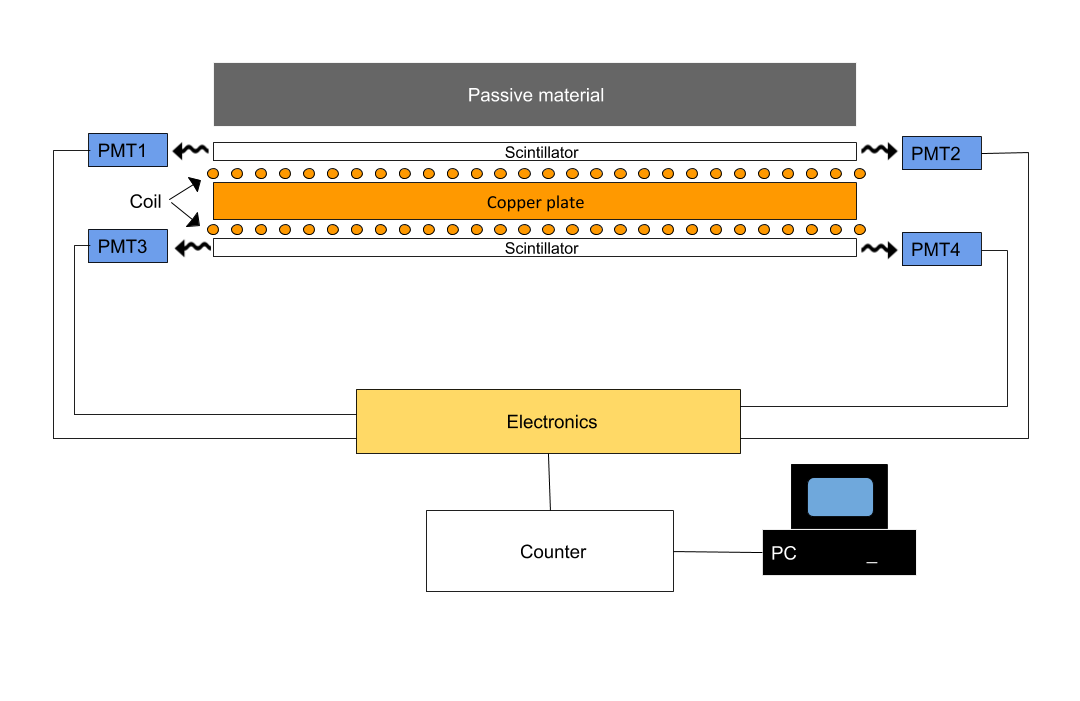
\includegraphics[width=\linewidth]{./fig/principle.png}
\caption{Illustration of the experimental apparatus.}
\label{fig:principle}
\end{figure}

The experiment's principle is described in Figure \ref{fig:principle}. The Copper target stops muons and is placed inside a magnetic field. The muon's lifetime is measured by looking at the time between a muon's stopping and the emission of a positron. The preferred direction and the Larmor frequency must also be registered in order to determine the magnetic moment. Particles are detected through scintillator plates. Scintillators are materials which, when ionized, will rearrange their electronic structures and emit photons at set energies. Those scintillators are isiolated from external luminous interference, connected to wave guides and then further to photomultipliers (here Photo-Multiplier-Tubes or PMTs), which then convert the light signal into an electronic one. The time differences are then saved on a PC. In other to provide further shielding to the experiment, a \SI{5}{\centi\meter} layer of dense and passive material (here lead) is added on top of the experiment.

A muon stop is experimentally defined as an electronic signal from the coincidence circuit of \textit{PMT}1 and \textit{PMT}2 but none from that of \textit{PMT}3 and \textit{PMT}4. Indeed an unstopped muon would traverse both scintillator layers and would thus register a signal in both coincidence circuits while a stopped one would traverse the top layer and not the bottom one. In logic language, a stopped muon would thus be written as:

\begin{equation}
(\text{\textit{PMT}1} \;\text{\textbf{AND}} \; \text{\textit{PMT}2}) \; \text{\textbf{AND}} \; (\overline{\text{\textit{PMT}3} \; \text{\textbf{AND}} \; \text{\textit{PMT}4}}).
\end{equation}

Two PMTs and a coincidence circuit are used so as to rule out random events and reduce electronic background. Muons generate strong photon bursts that can be seen by both PMTs. A muon decay is defined in the same way as a muon stop meaning that when a particle is sent downwards, it isn't registered, leading to a loss in statistics.

Nevertheless, this logic circuit is used because there would otherwise be no spatial resolution and thus no way to determine the muon spin which is needed for the magnetic moment determination. Since muon stops and decays are registered as the same signal, the two events need to be separated through their sequence:

\begin{itemize}
\item A muon decay is a stochastic process which thus is distributed according to an exponential probability distribution. For an average lifetime of $\tau=\SI{2.2}{\micro\second}$ we get a half-life $\lambda=\frac{\tau}{\ln(2)}\simeq \SI{1.5}{\micro\second}$, therefore $99\%$ of muons decay after $\SI{10}{\micro\second}$.
\item Due to the low vertical radiation intensity, the average distance between two muons is $\sim\SI{10}{\second}$ which is about 10 times the $\SI{12.5}{\micro\second}$ readout length. This reduces the likelihood of two overlapping events.
\end{itemize}

Thus, an event is identified as a muon-stop if and only if a second event takes place in the next \SI{12.5}{\micro\second} which then defines a decay. All other events are discarded.


\section{Target and B-field}

Muon are captured in a \SI{1}{\meter} long, \SI{50}{\centi\meter} wide and \SI{2.5}{\centi\meter} thick copper plate. Copper as a material has the following advantages justifying its use:

\begin{itemize}
\item It is slightly diamagnetic ($\chi_{\text{m}}=-7.4 \cdot 10^{-6}$) and thus has little influence over the magnetic field.
\item Its thickness allows it to effectively stop muons.
\item The muons are not depolarized by the formation of muonium.
\end{itemize}

The coil used in this experiment is \SI{1}{\meter} and composed of 456 loops. The calibration curve in Figure \ref{fig:magcal} shows the need for $\SI{10}{\ampere}$ for $\SI{48}{\gauss}$ (calibration $B[Gauss]=\SI{4.72}{\text{I}}$) and thus, a $\SI{4.1}{\mega\hertz}$ Larmor Frequency $\omega_{\text{L}}$. This corresponds to a period $T=\frac{2\pi}{\omega}$ so $\sin \SI{1.5}{\micro\second}$, which, with a time resolution of $\SI{0.05}{\micro\second}$ and a window of $\SI{12.5}{\micro\second}$, such as in this experiment, theoretically 7-8 periods should be observed.

\begin{figure}[htbp]
\centering
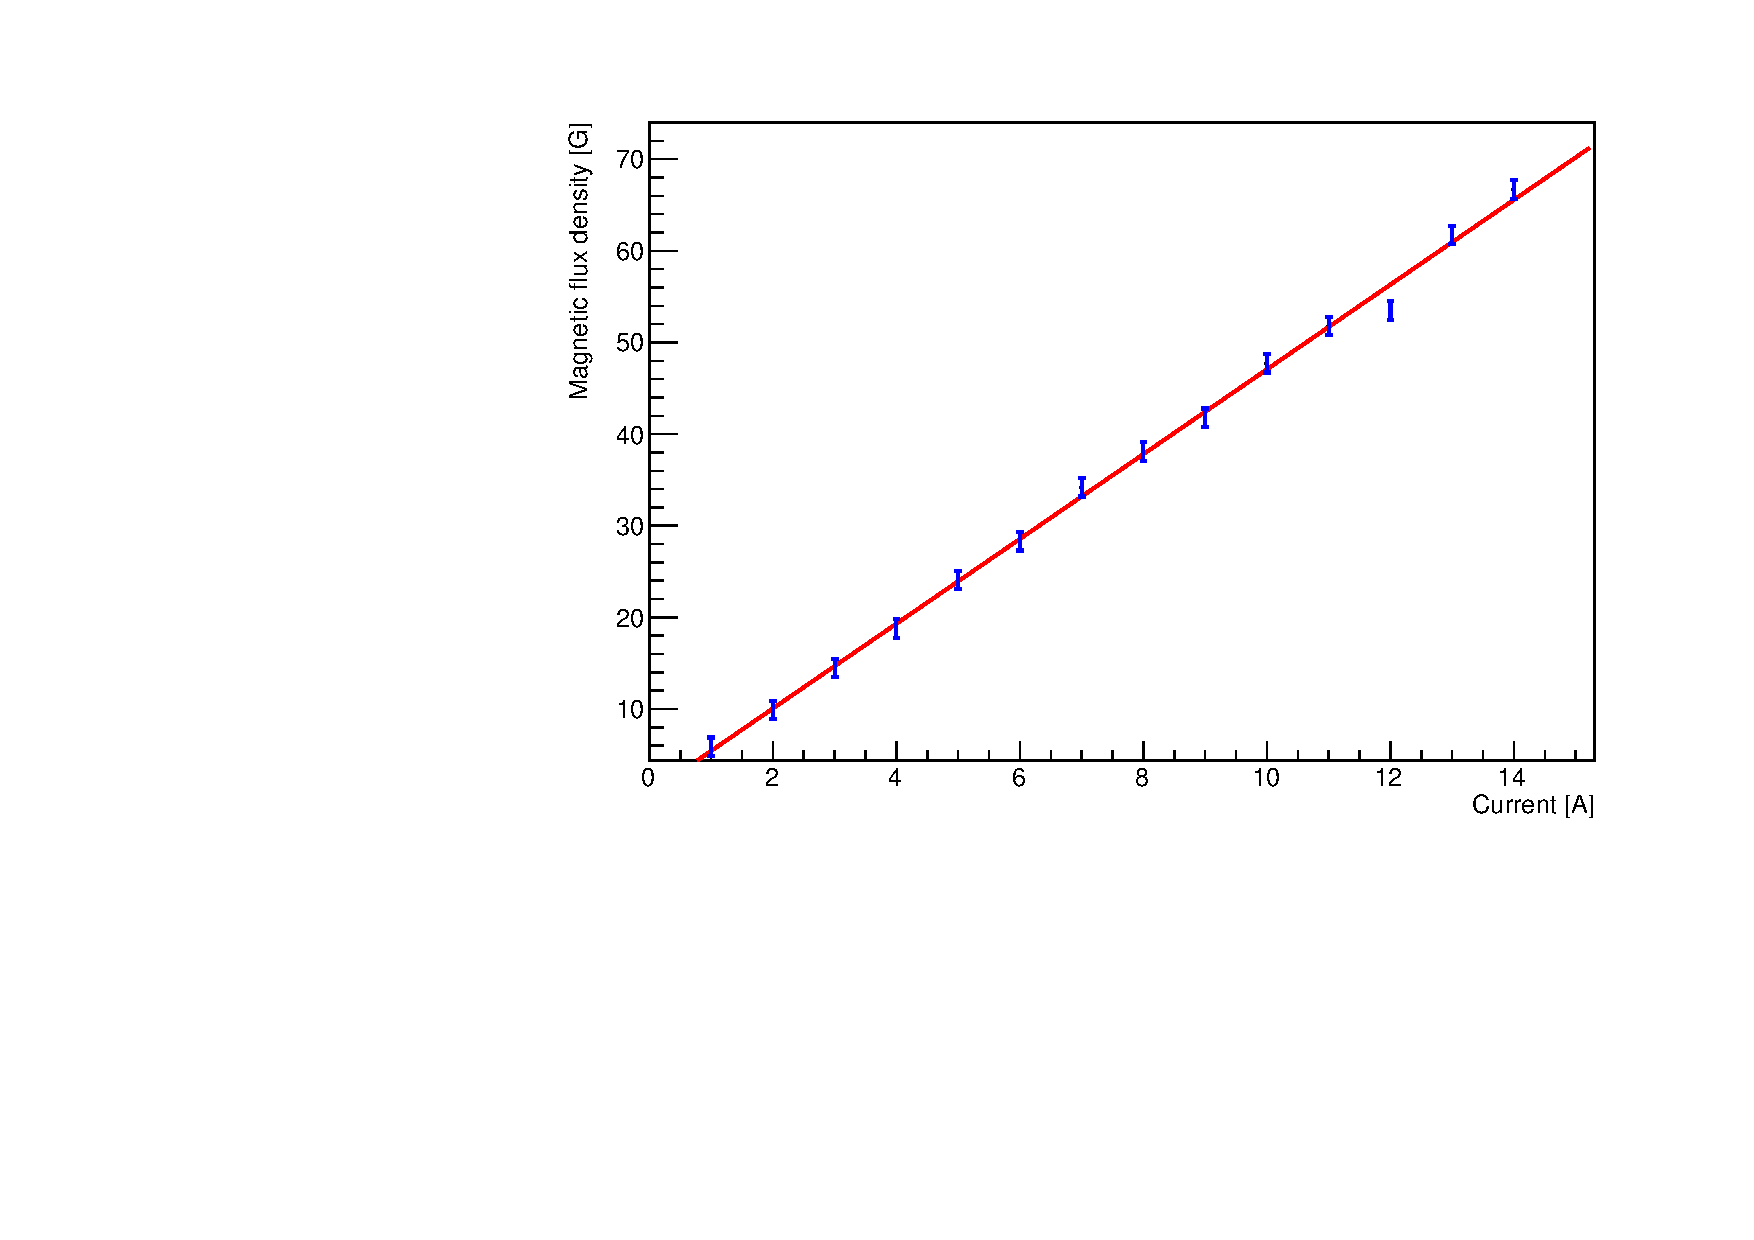
\includegraphics[width=0.7\linewidth]{./fig/magcal.pdf}
\caption{Calibration curve of the magnetic field as measured with a fluxgate compass.}
\label{fig:magcal}
\end{figure}


The magnetic field must however be homogenous enough that two muons stopped at different locations don't have too big of a phase difference. If the relative phase difference should be $\Delta\omega T \leq 0.3$, with $T$ being the measurement period (i.e. \SI{12.5}{\micro\second}). In this case, equation \ref{eq:larm} implies that the homogeneity of the B-field at \SI{48}{\gauss} must satisfy $\frac{\Delta B}{B}\leq 0.008$. If one uses the law of Biot-Savart to compute the magnetic field, they would find $\frac{\Delta B}{B}=0.013$. An additional \SI{10}{\centi\meter} long correction coil at each end of the main coil improves the value to 0.008. Calculations with different current values show that this value represents an absolute minimum for this arrangement and is achieved precisely when the correction coil current is half of that of the main coil. The secondary coils are thus connected in parralel to each other and in series with the main one as shown in Figure \ref{fig:coil}.

\begin{figure}
\centering
   \begin{subfigure}[t]{0.49\linewidth}
  \centering
   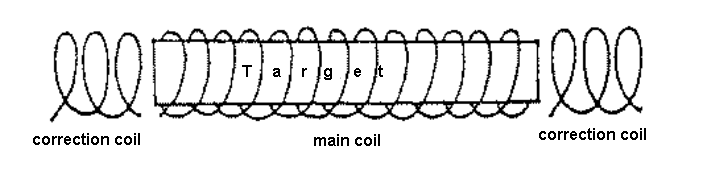
\includegraphics[width=\linewidth]{./fig/coil1.png}
  \caption{}
\label{sfig:coil1}
  \end{subfigure}
   \begin{subfigure}[t]{0.49\linewidth}
  \centering
   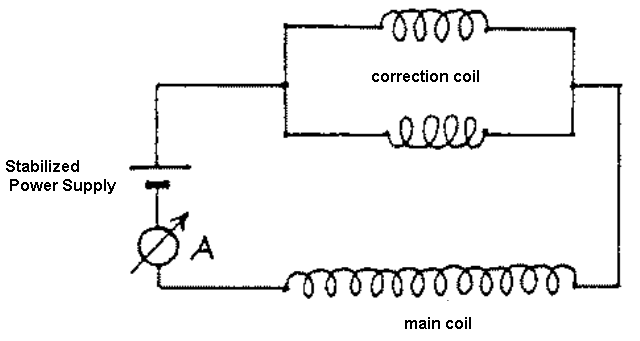
\includegraphics[width=\linewidth]{./fig/coil2.png}
  \caption{}
\label{sfig:coil2}
  \end{subfigure}
\caption{(a) Magnetic coil structure. (b) Magnetic coil circuit.}
\label{fig:coil}
\end{figure}

\begin{figure}
\centering
 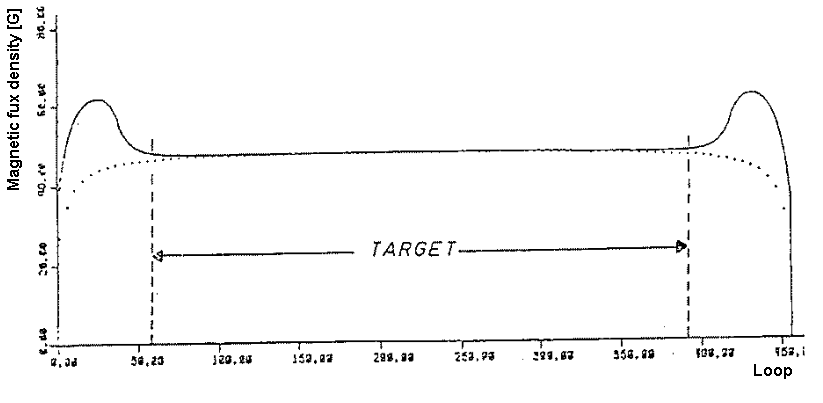
\includegraphics[width=\linewidth]{./fig/coillength.png}
\caption{Magnetic field as calculated along the coil at \SI{10}{\ampere}.}
\label{fig:fieldstr}
\end{figure}

\begin{figure}
\centering
 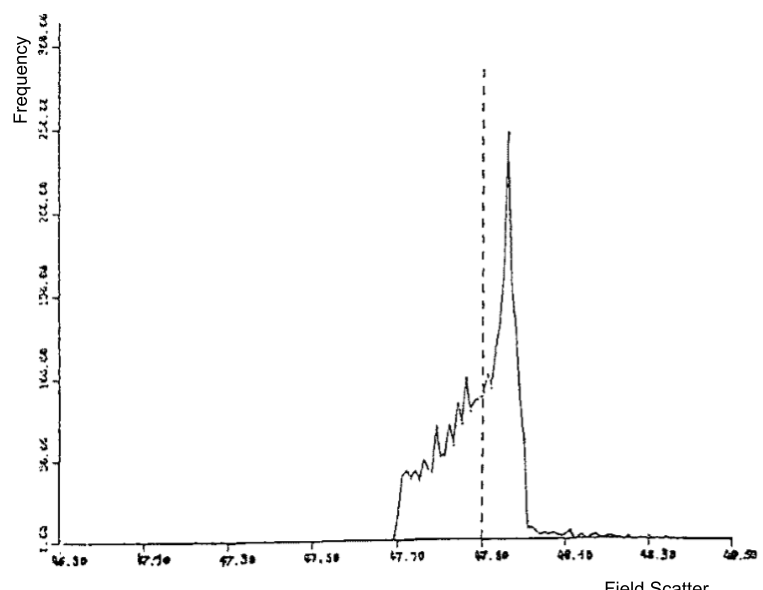
\includegraphics[width=\linewidth]{./fig/fieldscat.png}
\caption{Scatter of the B-field as calculated along the coil axis for a \SI{10}{\ampere} current. The dotted line represents the average scatter.}
\label{fig:fieldscat}
\end{figure}

The homogenity of the magnetic field is shown in Figures \ref{fig:fieldstr} \ref{fig:fieldscat}.
The temporal stability of the magnetic field's current is ensured through a stabilized power supply up to $0.5 \%$. The deterioration of $\frac{\Delta B}{B}$  by a further 0.005 such as to not observe the muon's polarization over the measurement period of \SI{12.5}{\micro\second}. In order to cool the coil, which is always powered at \SI{10}{\ampere}, a ventilator, which \textbf{always needs to be turned on when the B-field is in use}, is used.

\section{Particle detection apparatus}

The scintillators above and below the copper target are of type NE110 (organic scintillator) have a surface of $90 \times \SI{45}{\centi\meter\squared}$. As the ionizing particles pass through the scintillator, the molecular electron states are being excited, this leads to de-excitation with emission of UV light. Since the absorption length of this UV light is very short, it will be absorbed by another scintillator atom which will lead to a similar electronic process and the isotropic emission of another, shorter wavelength fluorencence photon. It is thus also called a wavelength shifter. The fluorescent decay time is of the order of $\SI{e-10}{\second}$. In order to reduce loss of signal, the scintillator surface is polished and covered in aluminized foil, allowing photon reflexion and limitingphoton escape. In other to deal with background from ambient light, photographic paper covered in black foil forms an outer layer of the scintillator units.

\section{The photomultiplier}

The light produced in the scintillators is guided in a plexiglas waveguide to a photomultiplier. A photomultiplier is an electronic detector used to convert light into electrons. The photomultipliers used here are Photo-Multiplier-Tubes (PMT) shown in Figure \ref{fig:PMT}, a widely used technology for light detection. The photomultiplier tube is based on a thin vapor-deposited conducting layer photocathode which converts photons to electrons via the photoelectric effect, these electrons are then passed through a focusing electrode directing them towards a dynode circuit serving to amplify the electron signal via secondary emission \cite{Dekker1981}. Each dynode is held at at slightly higher ($\sim \SI{100}{\volt}$) potential than the preceding one. When an electron strikes a dynode, it will cause emission of low energy electrons which will then be accelerated towards the next dynode. The geometry of the dynode circuit is such that a cascade occurs with an exponentially increasing number of electrons being produced at each dynode. The final dynode is connected to an anode. At this stage, a large number of electrons reach the anode, it will thus create a sharp rising edge which is an easy analog signal to detect. The voltage distribution in the dynodes is done through a voltage divider circuit. The photocathode is generally held at a negative high voltage of order 1000 V, while the anode is very close to ground potential. The capacitors across the final few dynodes act as local reservoirs of charge to help maintain the voltage on the dynodes while electron avalanches propagate through the tube. It should be noted that the design shown in Figure \ref{sfig:PVD} is only an example as many different such circuits exist.

\begin{figure}
\centering
   \begin{subfigure}[t]{0.49\linewidth}
  \centering
   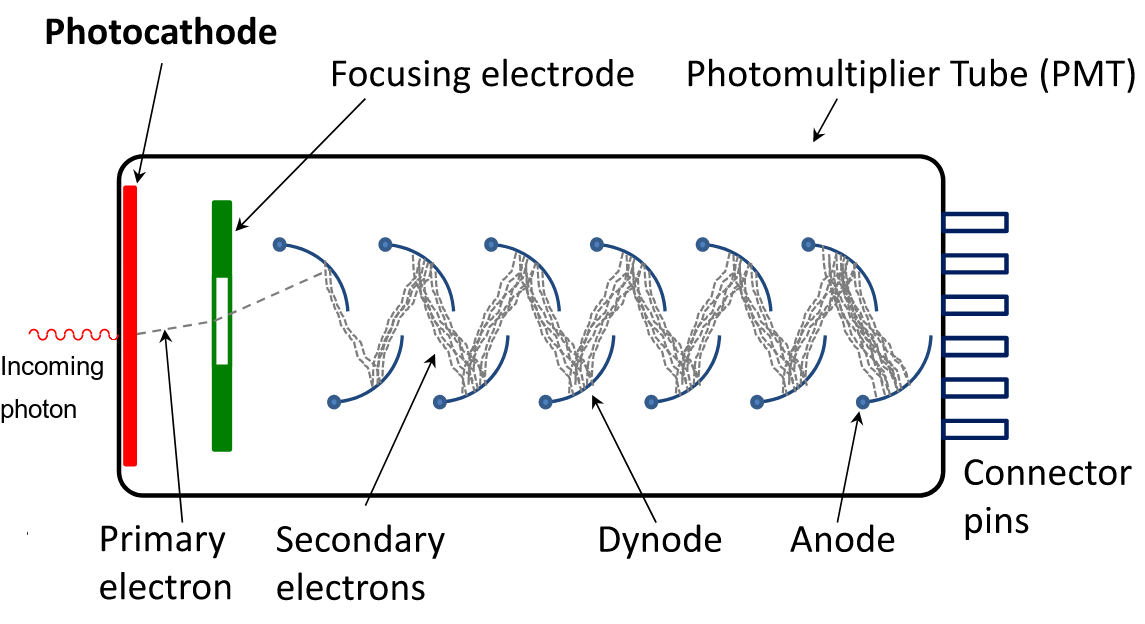
\includegraphics[width=\linewidth]{./fig/PMT.png}
  \caption{}
\label{sfig:PMT}
  \end{subfigure}
   \begin{subfigure}[t]{0.49\linewidth}
  \centering
   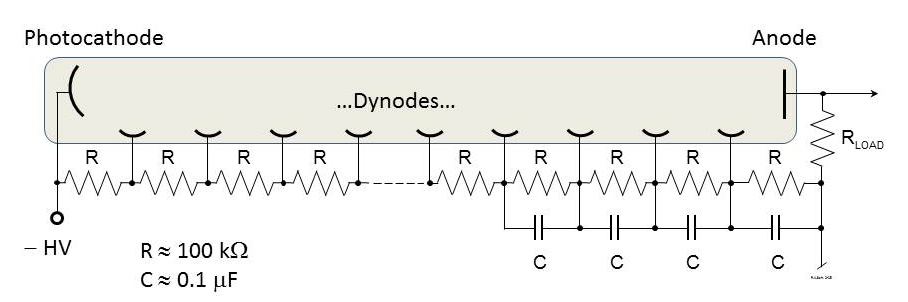
\includegraphics[width=\linewidth]{./fig/PMT_Voltage_Divider.jpg}
  \caption{}
\label{sfig:PVD}
  \end{subfigure}
\caption{(a) PMT schematic illustration. (b) PMT example voltage divider circuit \cite{wiki}.}
\label{fig:PMT}
\end{figure}


\section{Electronics}

\subsection{Introduction to signal electronics}

Electronics have historically worked around analog signals. These signal are the products of direct physical effects (typically electron/ion drift reaching the anode/cathode and creating a current). An analog signal is thus a continuous (sinusoidal) wave which is changing over a time period. They are typically described by their amplitude, period (or equivalently frequency) and phase, they have no fixed range and as a result are more unstable. A good example of an analog signal is the human voice which can modulate it's amplitude (volume), frequency (pitch) and phase (spacing) to transmit information. 



With the introduction of vacuum tubes and logic circuits, it became possible to produce and process binary signals. These function around sharp rising and falling edge signals, so-called gate functions which (in an ideal scenario) instantly pass from a reference, fixed, low voltage level (usually \SI{0}{V}) to a reference, fixed, high voltage. The corresponding electronics is then able to reckognize the change of voltage and act accordingly through boolean algebra of varying complexity. Digital signals are represented through bit rates and bit intervals, have a very well-defined and limited range (such as 0 and 1). They are as a result less prone to distortion and interference. Computers are among the best examples of digital signal carriers.


\subsection{Experiment logic}


The PMTs emit short, fast, subsequent (analog) electronic impulses, the electronics are used to discriminate muon-stop signals. This happens with a coincidence circuit. A coincidence can be seen as a an "electronic binary operator" (through an \textbf{AND} gate, thus ), it thus takes two signals as inputs which in the case of the Nuclear Instruments Module (NIM), take gate signals with binary values of \SI{700}{\milli\volt} (logical 1/\textbf{TRUE}) or \SI{0}{\volt} (logical 0/\textbf{FALSE}). It provides a fixed output based on the mode of operation either a gate signal or a logical 0. The coincidence can be operated as \textbf{AND} ($\odot$), \textbf{OR} ($\oplus$), \textbf{NAND} (=$\overline{\text{\textbf{AND}}}$) or \textbf{NOR} ($=\overline{\text{\textbf{OR}}}$). The output signal depends on the input algebra logic which can be found in Table \ref{tab:log}.

The conditions for a muon stop or decay from Figure \ref{fig:principle} can be written:

\begin{equation}
\big(\text{PMT}1 \odot \text{PMT}2\big) \odot \big(\overline{\text{PMT}1} \oplus \overline{\text{PMT}2}\big).
\end{equation}

The first block represents a logical \textbf{AND} while the second one represents a logical \textbf{NOR} (see Table \ref{tab:log}). The entire logical circuit, including the \textbf{AND} is realized in the electronic circuit shown in Figure \ref{fig:elek} in coincidences 1,2 and 3. The logical units used to make coincidences require sharp rectangular gate (digital) pulses which is why the analog PMT signal is connected to discriminators after amplification. 


Similarly to coincidences, discriminator output lengths can be varied. Discriminators also include the possibility to separate interference pulses (noise) from signal: they will only deliver a gate signal if the signal input exceeds a certain threshold which can be set. The rest of the circuit after coincidence 3 is used to set a counter to measure the decay time, from the start of a muon-stop (Reset) and stop at the subsequent event (interrupt) if this occurs within the fixed \SI{12.5}{\micro\second}. The counter reset and the \SI{12.5}{\micro\second} wide time window are implemented via the monoflop. A monoflop has one input ($s$) for start (as the reset is only used when operating as a flip-flop) and three outputs:

\begin{itemize}
\item $o$ (out) produces a gate output of variable length caused by an input and a \SI{0}{\volt} output otherwise.
\item $\overline{o}$ ($\overline{\text{out}}$) which produces an opposite signal to o.
\item $e$ (end) sends a short gate output of fixed length (per example \SI{10}{\nano\second}) when the output signal has ended.
\end{itemize}

\begin{figure}[htbp]
\centering
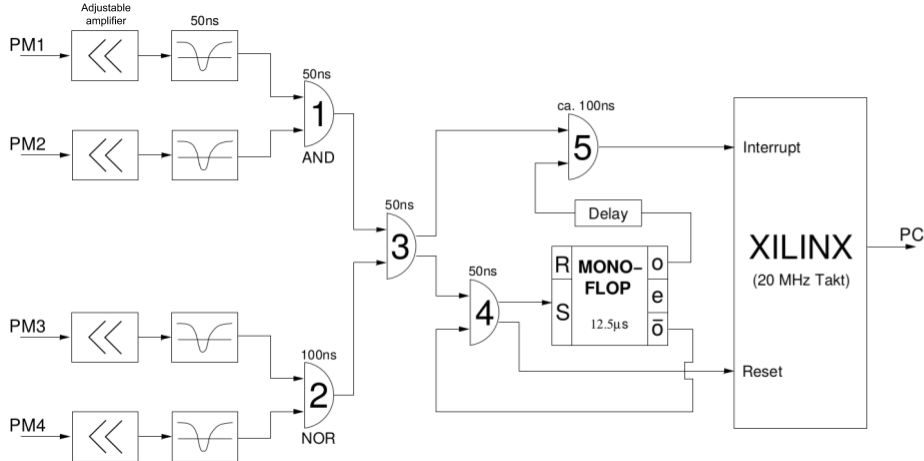
\includegraphics[width=0.7\linewidth]{./fig/electronicc.png}
\caption{Electronic circuit of the experiment.}
\label{fig:elek}
\end{figure}

\begin{table}
\begin{tabular}{|c|c|c|c|c|c|}
\hline
Input $\text{S}_1$ & Input $\text{S}_2$ & \textbf{AND} ($\odot$) output & \textbf{OR} ($\oplus$) output & \textbf{NAND} ($\overline{\text{\textbf{AND}}}$) output & \textbf{NOR} ($\overline{\text{\textbf{OR}}}$) \\ \hline
1 & 1 & 1 & 1 & 0 & 0 \\
1 & 0 & 0 & 1 & 1 & 0 \\
0 & 1 & 0 & 1 & 1 & 0 \\
0 & 0 & 0 & 0 & 1 & 1 \\ \hline
\end{tabular}
\caption{Coincidence logic table.}
\label{tab:log}
\end{table}


The monoflop open with a \SI{12.5}{\micro\second} gate for coincidence 5 and blocks coincidence 4 so that the reset switch isn't hit during the measurement period. Coincidence 5 is then ready for \SI{12.5}{\micro\second} to receive the second, supposedly delayed second signal from coincidence 3 and thus stop the counter.

The variable delay between monoflop and coincidence is achieved through an extra cable. It is crucial that signals from coincidence 3 nd the monoflop be perfectly spaced out since the start signal cannot be allowed to overlap with the gate so as to immediately trigger a reset. On the other hand, dead time between the start signal and the start of the gate (which is accepted as a stop) cannot take place either.

\section{Time measurement}

The time between the first, muon-stop, signal and the ensuing signal (muon decay) will be determined with a \textit{Time to Digital Converter} (TDC). This TDC is done with a \textit{Field Programmable Gate Array} (FPGA) from XILINX. An FPGA can be seen as an array of programmable logic blocks not unlike the coincidences described earlier. The blocks and their connections are programmed in by the user. Interactions with the outside world is done through I/O blocks. A network of programmable connections is available for connections between individual blocks.

The TDC is here programmed so as to function similarly to an 8-bit counter, which is reset through the aforementionned Reset-signal. Until the interrupt signal is received, the value of the counter is incremented by one unit for every XILINX board cycle. The clock frequency of the board is 20 MHz which corresponds to a counting unit of \SI{50}{\nano\second} and thus yields a maximum counted time difference is \SI{12.8}{\micro\second}. If the interrupt signal is received within this time, the counter's value is readout by the software on the connected PC	and converted into a time value.


\section{Data acquisition with the PC}

4-5 \si{events\per\minute} are expected. This counting rate thus requires to extend the measurement period to a week in order for enough statistics to be gathered. The DAQ program works as follows: when the XILINX obtains a valid event, its counter's value is sent to the PC and converted there into a time value. This value is then histogrammed which has 256 bins of \SI{50}{\nano\second}, corresponding to the range of all possible values that can be outputed by the TDC. The time measurements are then plotted and saved for every event (allowing for data recovery in the case of a crash or the like). The data is written into files which can be then easily be read-out. The DAQ software is in german but a measurement can be started by going into \textit{Messung}$\rightarrow$\textit{Beginnen} and ended through \textit{File}$\rightarrow$\textit{Beenden}, the measurement GUI and window can be found in Figure \ref{fig:MP}.

\begin{figure}
\centering
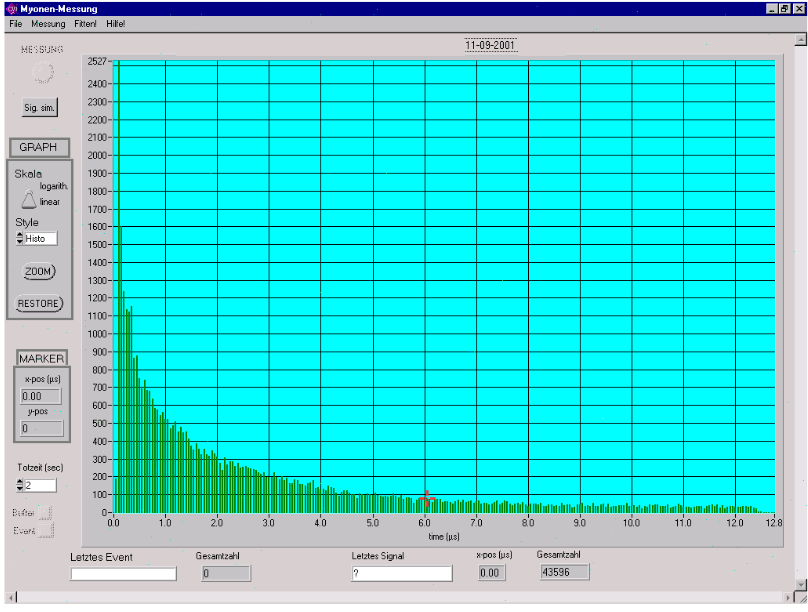
\includegraphics[width=\linewidth]{./fig/MP.png}
\caption{Measurement software window.}
\label{fig:MP}
\end{figure}

    \chapter{Measurement and analysis}

\section{Preparatory measurements}

Before the actual measurement can be understaken, a couple of preparations must be made such as setting the PMT voltages, the discriminator thresholds and finally testing the electronics with simulated pulses.

\subsection{Setting the counter}

The discriminator's rectangular pulse widths are set to \SI{50}{\nano\second}, this provides long enough pulses for the coincidences while also minimizing the amount of random coincidences which arise from the overlap of two successive pulses due to their finite width. The Number $N_{\text{z}}$ of random coincidences is a function of the pulse width $T_{\text{i}}$ and the number of impulses according to:

\begin{equation}
N_{\text{z}}=N_1 N_2(T_1+T_2),
\end{equation}

where the counting rate of the PMTs are to be determined. This is done by determining the expected muon rate. A well known figure for astroparticle experimentalists is that of \SI{1}{muon\per\minute\per\centi\meter\squared}, this means that for the scintiallator area of \SI{4000}{\centi\meter\squared}, the PMT and discriminators should be set such as to register approximately \SI{4000}{counts\per\minute}. This is fufilled approximately when the total counting rate is about \SI{6000}{\per\minute}. The counting is done with a dedicated counter ("Scaler") which counts logical pulses for a user-selected period.

The number of random coincidences is thus expected to be:

\begin{equation}
N_{\text{z}}=\frac{6000^2}{60^2 \: \si{\second\squared}}\SI{100e-9}{\second}\sim 1.0 \cdot \SI{e-3}{\per\second},
\end{equation}

which corresponds to $\sim \SI{0.06}{events\per\minute}$ which is negligible when compared to the expected rate of $\SI{4000}{events\per\minute}$.

An expectation value for the effective count rate can then be computed: around 4000 muons are expected to cross the scintillator every minute, the efficiency of the setup is $\sim 50\%$, muons with energies between $601$ and $\SI{617}{\mega\electronvolt}$ are stopped by the copper target. The energy spectrum shown in Figure \ref{fig:shift} implies that about 4-5 events should be recorded every minute. This expectation is observed to be in good agreement with observations.

\section{Electronic test with simulated pulse}

A muon decay can be tested with the help of a pulse generator. The generator emits two short pulses with pre-set time intervals (which can be set from \SI{10}{\nano\second} to \SI{1}{\second}). The pulses must be passed through discriminators 1 and 2, such as their time difference trigger the counter. If the distance is, per example \SI{5}{\micro\second}, the counter should display 100 (channels), one channel corresponding to \SI{0.05}{\micro\second}. If the double pulses are repeated frequently, the deviation shouldn't exceed $\pm\SI{1}{\text{channel}}$. If there is a constant difference in the time interval (``offset''), this can be corrected later.



    \chapter*{Experiment schedule}

\section{On the day of the experiment}

\begin{itemize}

\item Preliminary test: Elementary particles, cosmic rays, muon production, polarization and decay, experiment apparatus, decay spectrums.

\item Setting up the electronics and PMT voltage, discriminators and gate lengths.

\item Testing the electronics and calibrating the time measurement through simulated muons using the pulse generator.

\item Starting the measurement.
\end{itemize}

The measurement takes one week. The ensuing analysis is to be done at home, using whichever tools are seen fit. It is recommended that students review the functionning of the electronics, especially coincidence units and the monoflop.



    \chapter*{Annex}

\section{Electronics description}


The different pieces of electronics used in this experiment are described here.

\subsection{Amplifier}

Amplifiers are an electronic device which is used to increase the amplitude of a signal through modulation of output voltage or current. The ratio between the output amplitude and the input amplitude is called the \textit{Gain} ($G$). An example is shown in Figure \ref{fig:amplisin}

\begin{figure}[htbp]
\centering
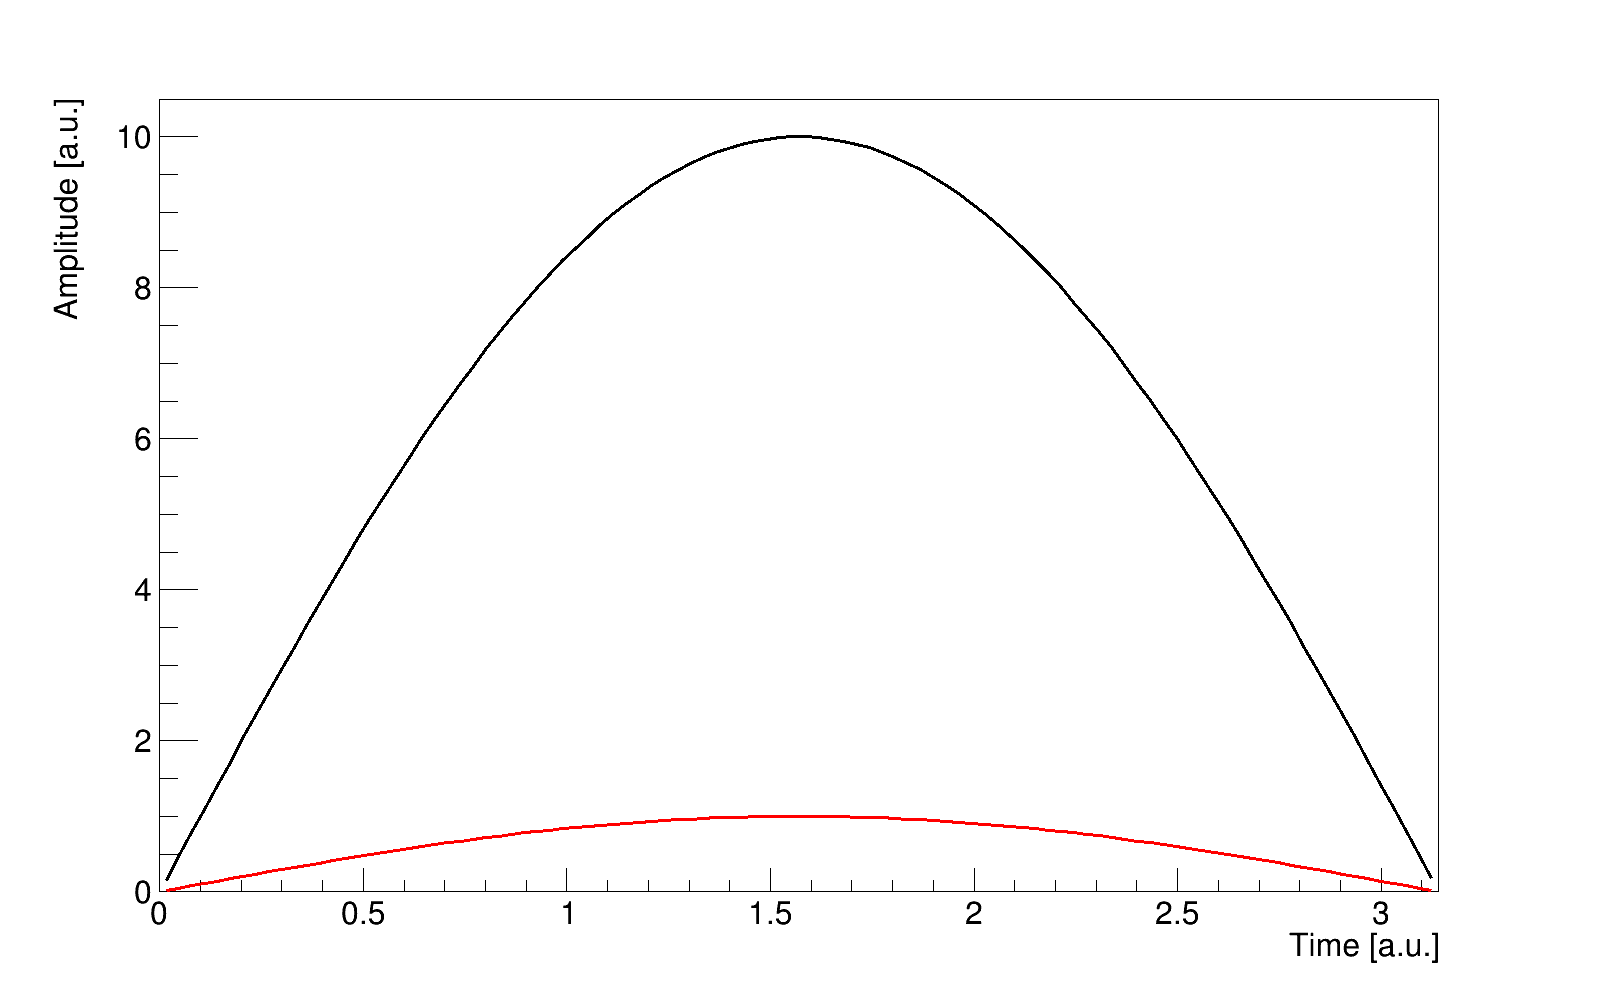
\includegraphics[width=0.7\linewidth]{./fig/amplisin.png}
\caption{Signal wave (red) and its ten-fold ($G=10$) amplified counterpart (black).}
\label{fig:amplisin}
\end{figure}

The experiment's amplifiers' gains can be tuned using a screwdriver on the holes left of the inputs.


\subsection{Discriminators}


Discriminators are an electronic Analog to Digital Converter (ADC). They produce a digital output when the signal fulfills certain conditions. If and when that is the case, a discriminator releases a single digital signal. Discriminators generally fall in one of two catergories: \textit{Leading Edge Discriminators} or \textit{Constant Fraction Discriminators} depending on which conditions they use to accept an analog signal:

\begin{itemize}

\item A leading edge discriminator only looks at the leading edge of signal, if the signal reaches the threshold level the logic pulse is emitted. This however can lead to \textit{walk}: time variance dependent on the size of the signal. This can increase difficulty in adjusting the timing information in the rest of the setup, and makes it impossible to obtain accurate timing information later. Thus, the constant fraction discriminator was created.

\item A constant fraction discriminator (CFD) works by looking at the entire signal and emits the logical pulse when the input signal reaches a certain fraction of its peak value. In this way a signal that has a wide time variance can be narrowed significantly using a leading edge discriminator.

\end{itemize}

The rate in the experiment being low and the timing not being critical at this stage of the circuit, the discriminators used here are of LE type.

\subsection{Monoflop unit}

Monoflops (shortened for \textit{Monostable Multivibrators}) are a sequential logic circuit that takes an input, two outputs and a clock unit (which may be seen as an extra input). The sequential part of the circuit (the clock) are continuous square function generators at a fixed frequency as shown in Figure 

\begin{figure}[htbp]
\centering
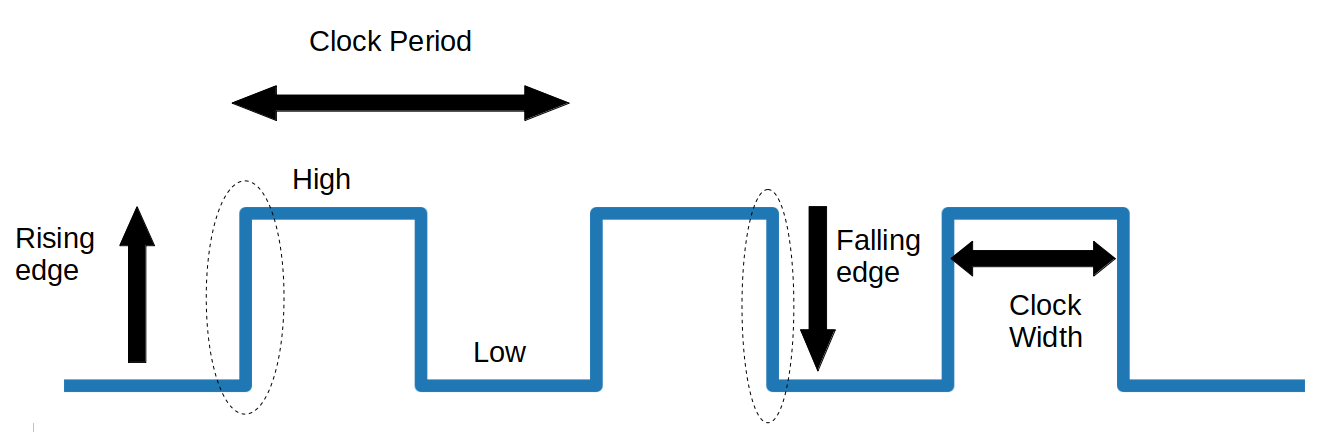
\includegraphics[width=0.7\linewidth]{./fig/rising.png}
\caption{Clock parameters.}
\label{fig:rising}
\end{figure}

Such sequential logic circuits using clock signals for synchronization depend on their frequency and therefore the clock pulse width to activate their switching action. Sequential circuits can also change their switching state using either the rising edge, falling edge, or both edges of the clock signal.

Monostable Multivibrators or “one-shot” pulse generators are generally used to convert short, sharp pulses into much wider ones for timing applications. Monosflops generate a single output pulse, either $1$ or $2$, when a suitable external trigger signal or start pulse T is applied.

This trigger pulse signal initiates a timing cycle which causes the output of the monostable to change state at the start of the timing cycle, ($t_1$). The ouput remains in this second state until the end of the timing period, ($t_2$) which is determined by the time constant of its timing capacitor, $CT$ and the resistor, $RT$.

The monostable multivibrator now stays in this second timing state until the end of the RC time constant and automatically “resets” or returns itself back to its original (stable) state.

In this experiment, the monoflop utilizes its clock to count over a set period of time, until it either received a second input (signaling a muon decay) or time runs out (no decay is seen/background).






\bibliography{bib/Experiment41}
\bibliographystyle{abbrv}
\end{document}

